\documentclass[11pt,a4paper]{article}
\usepackage[T1]{fontenc}
\usepackage[utf8]{inputenc}
\usepackage{lmodern}
\usepackage{microtype}
\usepackage[margin=30mm]{geometry}
\usepackage{amsmath,amssymb,amsthm,mathtools}
\usepackage{mathrsfs}
\usepackage{enumitem}
\usepackage{needspace}
\usepackage{tikz}
\usetikzlibrary{arrows.meta,calc,positioning}
\usepackage[nottoc,notlof,notlot]{tocbibind}
\usepackage{xcolor}
\definecolor{linkblue}{RGB}{24,62,107}
\usepackage[colorlinks=true,linkcolor=linkblue,citecolor=linkblue,urlcolor=linkblue,
  pdftitle={A local Penrose inequality for conformal perturbations of Schwarzschild--anti-de Sitter data},
  pdfauthor={OpenAI}]{hyperref}
\usepackage[nameinlink,noabbrev]{cleveref}
\usepackage{bookmark}
\numberwithin{equation}{section}
\newtheorem{theorem}{Theorem}[section]
\newtheorem{proposition}[theorem]{Proposition}
\newtheorem{lemma}[theorem]{Lemma}
\newtheorem{corollary}[theorem]{Corollary}
\theoremstyle{definition}
\newtheorem{definition}[theorem]{Definition}
\newtheorem{remark}[theorem]{Remark}
\crefname{theorem}{Theorem}{Theorems}
\crefname{proposition}{Proposition}{Propositions}
\crefname{lemma}{Lemma}{Lemmas}
\crefname{corollary}{Corollary}{Corollaries}
\crefname{definition}{Definition}{Definitions}
\crefname{remark}{Remark}{Remarks}
\crefname{section}{Section}{Sections}
\crefname{equation}{Equation}{Equations}
\newcommand{\eps}{\epsilon}
\newcommand{\dd}{\mathrm{d}}
\newcommand{\AH}{\mathrm{AH}}
\newcommand{\II}{\mathrm{II}}
\newcommand{\tf}{\circ}
\newcommand{\R}{\mathbb R}
\newcommand{\N}{\mathbb N}
\DeclareMathOperator{\Ric}{Ric}
\DeclareMathOperator{\Hess}{Hess}
\DeclareMathOperator{\Div}{div}
\DeclareMathOperator{\tr}{tr}
\DeclareMathOperator{\scal}{Scal}
\DeclareMathOperator{\grad}{grad}
\DeclareMathOperator{\sym}{sym}
\DeclareMathOperator{\supp}{supp}
\setlist[enumerate]{label=\textup{(\roman*)},leftmargin=2em}
\setlength{\emergencystretch}{2em}
\allowdisplaybreaks[1]
\title{A local Penrose inequality for conformal perturbations\\
of Schwarzschild--anti-de Sitter data}
\author{OpenAI}
\date{October 5, 2026}
\begin{document}
\maketitle
\begin{abstract}
We prove the asymptotically hyperbolic Penrose inequality for sufficiently
small maximal vacuum conformal perturbations of a positive-mass
Schwarzschild--anti-de Sitter exterior, for every fixed decaying
transverse-traceless seed and every solution branch satisfying the stated
decay and mass assumptions. The bound uses the area of the marginally
outer trapped boundary itself; it requires neither outermostness nor
outer area-minimization, and no bulk-versus-boundary domination condition.
For sufficiently small positive parameters, equality holds for radial
seeds and the inequality is strict otherwise.
\end{abstract}
\tableofcontents
\clearpage
\section{Introduction}\label{sec:introduction}

The Penrose inequality relates the total mass of gravitational initial
data to the area of a black-hole boundary. Its original formulation arose
from the relation between gravitational collapse and cosmic
censorship~\cite{Penrose1973}. In the asymptotically flat,
time-symmetric setting it was proved by Huisken and Ilmanen for a
connected horizon and by Bray for the total area of possibly disconnected
horizons~\cite{HuiskenIlmanen2001,Bray2001}. For negative cosmological
constant, the Schwarzschild--anti-de Sitter family suggests the
three-dimensional inequality
\begin{equation}\label{eq:intro-penrose}
 m_{\AH}\geq
 \sqrt{\frac{A}{16\pi}}\left(1+\frac{A}{4\pi}\right),
\end{equation}
when the cosmological constant is normalized to $-3$.
Here $m_{\AH}$ is the Lorentz norm of the hyperbolic mass covector.
In the outermost, outer area-minimizing formulation of
Corollary~\ref{cor:penrose}, $A$ is the least enclosing area of the
future marginally outer trapped boundary.

We prove \eqref{eq:intro-penrose} for a local conformal class of
maximal vacuum data with a marginally outer trapped boundary.
The background is a time-symmetric Schwarzschild--anti-de Sitter
exterior of arbitrary positive mass. One fixes a smooth decaying
transverse-traceless (TT) tensor $q$ and considers any solution branch of
the conformal constraint equation with conformal second fundamental
form $\eps q$. The parameter interval in the result may depend on this
fixed seed and branch. Theorem~\ref{thm:main} imposes neither symmetry
nor an additional comparison between the size of the seed in the
interior and at the boundary.

This setting is closely related to the perturbative theorem of
Khuri and Kopi\'nski~\cite[Theorem~2]{KhuriKopinski2023}.
Their sufficient condition requires the static-lapse-weighted integral
of the squared seed norm to dominate a multiple of the squared $H^1$
norm of its normal component on a domain containing the boundary;
see their Equation~(2.5). Both sides scale quadratically when the seed is
multiplied by $\eps$, so shrinking $\eps$ alone does not remove that
condition. The argument below replaces it by a sharp TT boundary
identity and treats the equality directions of the resulting
quadratic estimate. It thereby proves the fixed-seed local form
of the Penrose inequality in this conformal class without the
domination hypothesis. In particular, it applies when the boundary
is outermost and outer area-minimizing, as in the usual local
Penrose formulation.

Two related geometric ingredients have established precedents.
The hyperbolic mass covector and its covariance are studied by
Chru\'sciel and Herzlich~\cite{ChruscielHerzlich2003}.
Neves and Tian construct constant mean curvature (CMC) foliations near
infinity under
positive-mass Schwarzschild--anti-de Sitter asymptotic
hypotheses~\cite{NevesTian2009}; Ambrozio uses CMC foliations to prove
a local Riemannian Penrose inequality near
Schwarzschild--anti-de Sitter~\cite{Ambrozio2015}.
We derive directly the mass and CMC identities needed here.
Only finite Taylor families of surfaces are used, so the proof
does not require an actual global CMC foliation for a nonzero
parameter.

\subsection*{The mechanism of the proof}

Write $\mathfrak D_q(\eps)$ for the difference between the two
sides of \eqref{eq:intro-penrose}, with $A$ the boundary area.
In the notation of Section~\ref{sec:setting}, $g_0$ is the background
metric of mass $m_0$, $s$ is proper radial distance, $r(s)$ is the
area radius, and $N=r'(s)$ is the static lapse.
The constant and linear deficit coefficients vanish. The quadratic
calculation combines a CMC
Hawking-mass identity with the static TT identity
\[
 NQ(v)=\sym\nabla(N\,\dd v-v\,\dd N),
 \qquad Q(v)=\nabla^2v-v(\Ric_{g_0}+3g_0).
\]
After the boundary area correction, the quadratic coefficient is a
sum of nonnegative terms (Proposition~\ref{prop:quadratic}). Its kernel
is the four-dimensional space of tensors $Q(v)$, where
$(\Delta_{g_0}-3)v=0$, $v$ decays, and $v|_S$ contains only constant
and degree-one spherical harmonics (Corollary~\ref{cor:kernel}).

The degree-one directions are a real obstruction to concluding from
second order. They have zero first-order shear and lapse fluctuation,
and a radial component can make their boundary normal component
nonnegative. We remove their first extrinsic-curvature coefficient
by a change of spacetime slice at the level of finite Taylor expansions. The
resulting quartic coefficient is again a sum of nonnegative terms.
If it vanishes, the changed metric must be a round warped-product
jet through second order. Conformality of the original branch then
forces the radial profile $V(s)$ of the degree-one part of $v$ to satisfy
(with primes denoting $s$-derivatives)
\[
 \left(V'-\frac{r'}rV\right)^2=\frac{6m_0}{r^3}V^2.
\]
This is incompatible with a nonzero decaying profile. Thus the
quartic coefficient is strictly positive in every nonradial
quadratic-null direction (Proposition~\ref{prop:quartic}). The remaining
radial directions satisfy an exact conserved-mass identity
(Proposition~\ref{prop:radial}).

Three parts of the method may be useful beyond this application:
the sharp static TT boundary square; the passage from CMC surface
jets to a positive mass-coefficient identity by integrating first
at finite radius; and the use of a null boundary transport together
with a change of slice to detect a quartic obstruction. Analytically,
an exact Green formula converts the derivative-defined mass into
convergent integrals. It allows actual remainder estimates in a
weighted function norm, and rotation averaging then covers seeds
with arbitrary angular dependence. Proposition~\ref{prop:expansions}
then identifies the finite Taylor calculations with the actual deficit.

The result concerns this fixed-seed local conformal problem.
No existence of a solution branch for every seed is asserted.
The proof does not use a general spacetime Penrose inequality,
a constrained extension through the boundary, or a global
spacetime development.

\section{Geometric setting and the theorem}\label{sec:setting}

Fix $m_0>0$, and let $a>0$ be the unique positive root of
$1+a^2-2m_0/a=0$. On
\[
 M=[0,\infty)\times S^2,\qquad S=\{0\}\times S^2,
\]
let
\begin{equation}\label{eq:background}
 g_0=\dd s^2+r(s)^2\sigma,\qquad
 r(0)=a,\qquad r'(s)>0\quad(s>0),\qquad
 (r')^2=1+r^2-\frac{2m_0}{r},
\end{equation}
where $\sigma$ is the unit round metric. The coordinate $s$ is smooth
at the boundary, and $n=\partial_s$ points from $S$ toward infinity.
On the end, $r=r(s)$ is a coordinate and
\begin{equation}\label{eq:hyperbolic-reference}
 b=\frac{\dd r^2}{1+r^2}+r^2\sigma
   =\dd\eta^2+\sinh^2\eta\,\sigma,\qquad
 \eta=\operatorname{arsinh}r.
\end{equation}
In particular, $r$ is asymptotic to a positive constant times $e^s$.

Our Laplacian is $\Delta=\Div\grad$, with nonpositive eigenvalues
on a closed manifold. The spaces $C^{k,\alpha}_\tau$ use the
hyperbolic metric $b$ in the end: the tensor and its covariant
derivatives through order $k$ are $O(e^{-\tau s})$, and the
correspondingly weighted $\alpha$-H\"older seminorms on unit
background balls are bounded. On a compact set we use ordinary
$C^{k,\alpha}$ regularity. This definition is equivalent to one
using hyperbolic distance.

Fix $0<\alpha<1$, $3/2<\tau<3$, and a smooth symmetric tensor
$q\in C^{1,\alpha}_\tau$, smooth up to $S$, satisfying
\begin{equation}\label{eq:tt-seed}
 \tr_{g_0}q=0,\qquad \Div_{g_0}q=0.
\end{equation}
Throughout the paper the seed $q$ is independent of $\eps$.
Suppose a smooth branch of positive solutions, defined for
$0\leq\eps<\eps_*$, satisfies
\begin{align}
 \Delta_{g_0}\phi_\eps
 &=\frac34(\phi_\eps^5-\phi_\eps)
   -\frac{\eps^2}{8}|q|_{g_0}^2\phi_\eps^{-7}
       &&\text{on }M,\label{eq:conformal-equation}\\
 \partial_s\phi_\eps
 &=\frac{\eps}{4}q_{ss}\phi_\eps^{-3}
       &&\text{on }S,\label{eq:conformal-boundary}\\
 \phi_0&=1,\qquad
 \phi_\eps-1\in C^{2,\alpha}_\tau,\qquad
 \|\phi_\eps-1\|_{C^{2,\alpha}_\tau}\longrightarrow0
       &&\text{as }\eps\longrightarrow0.\label{eq:branch}
\end{align}
No differentiability in stronger weighted spaces is assumed.
Set
\begin{equation}\label{eq:actual-data}
 g_\eps=\phi_\eps^4g_0,\qquad
 K_\eps=\eps\phi_\eps^{-2}q,\qquad
 A_\eps=|S|_{g_\eps}.
\end{equation}

\subsection{Mass and boundary conventions}

Let $x_i$, $1\leq i\leq3$, be the coordinate functions on the unit
sphere. Define $V_0=\sqrt{1+r^2}$, $V_i=rx_i$, and
$e_\eps=g_\eps-b$. We use the flux normalization
\begin{equation}\label{eq:mass-flux}
\begin{split}
 p_\mu(\eps)=\frac1{16\pi}\lim_{R\to\infty}
 \int_{\{r=R\}}\big[
 &V_\mu(\Div_b e_\eps-\dd\tr_b e_\eps)\\
 &+(\tr_b e_\eps)\dd V_\mu
      -e_\eps(\grad_bV_\mu,\cdot)
 \big](\nu_b)\,\dd A_b ,
\end{split}
\end{equation}
where $\nu_b$ points toward increasing $r$. All operators and the
area form in this formula are those of $b$. Assume that these
limits are finite and that the covector is future timelike for
all sufficiently small positive $\eps$. Thus
\[
 m_{\AH}(\eps)=\sqrt{p_0(\eps)^2-\sum_{i=1}^3p_i(\eps)^2}
\]
is the positive mass norm. This normalization gives $p_0(0)=m_0$
and $p_i(0)=0$. The $p_i$ are spatial components of the hyperbolic
mass covector, not angular momentum charges.

For a two-sided surface with unit normal $\nu$ toward the chosen
end, put
\[
 H=\Div_\Sigma\nu,\qquad
 \theta_+=H+\tr_\Sigma K.
\]
For a spacetime realization our convention is
$K(X,Y)=\bar g(\bar\nabla_Xn_{\mathrm{future}},Y)$;
in Gaussian normal coordinates this means $\partial_tg=2K$.
A future marginally outer trapped surface, or MOTS, has
$\theta_+=0$.

The standard conformal identities give
\begin{equation}\label{eq:constraints}
 \tr_{g_\eps}K_\eps=0,\qquad
 \Div_{g_\eps}K_\eps=0,\qquad
 R_{g_\eps}+6=|K_\eps|_{g_\eps}^2.
\end{equation}
Indeed, for a tracefree $q$ the divergence identity is
$\Div_{\phi^4g_0}(\phi^{-2}q)=\phi^{-6}\Div_{g_0}q$.
Also
\[
 R_{\phi^4g_0}
 =\phi^{-5}(-8\Delta_{g_0}\phi-6\phi)
 =-6+\eps^2\phi^{-12}|q|_{g_0}^2.
\]
The boundary $S$ is totally geodesic for $g_0$.
Its normal in $g_\eps$ is $\phi_\eps^{-2}\partial_s$, and
\begin{equation}\label{eq:boundary-mots}
 H_{g_\eps}(S)=4\phi_\eps^{-3}\partial_s\phi_\eps
       =\eps\phi_\eps^{-6}q_{ss},\qquad
 \tr_SK_\eps=-\eps\phi_\eps^{-6}q_{ss}.
\end{equation}
Consequently it is a future MOTS. Its mean curvature need not vanish.

\subsection{Statement}

Define
\begin{equation}\label{eq:deficit}
 b_*(A)=\sqrt{\frac A{16\pi}}\left(1+\frac A{4\pi}\right),
 \qquad
 \mathfrak D_q(\eps)=m_{\AH}(\eps)-b_*(A_\eps).
\end{equation}
A tensor is called \emph{radial} if it is invariant under every
rotation of the $S^2$ factor.

\begin{theorem}\label{thm:main}
For every background, fixed TT seed, and solution branch satisfying
\eqref{eq:background}--\eqref{eq:branch} and the mass assumptions
above, there is $0<\eps_0\leq\eps_*$ such that
\[
 m_{\AH}(\eps)\geq
 \sqrt{\frac{A_\eps}{16\pi}}\left(1+\frac{A_\eps}{4\pi}\right)
 \qquad(0\leq\eps<\eps_0).
\]
For all sufficiently small positive $\eps$, equality holds if the
seed is radial, and the inequality is strict otherwise.
\end{theorem}

The theorem makes no sign assumption on $q_{ss}|_S$.
It also does not require outermostness or outer area-minimization.
In particular it implies the following formulation with the usual
geometric boundary hypotheses. Here an enclosing surface separates $S$
from the end and bounds with $S$ a compact region. Write $A_{\min}(S)$
for the infimum of areas of smooth enclosing surfaces, allowing
disconnected competitors and $S$ itself.

\begin{corollary}\label{cor:penrose}
In addition to the hypotheses of Theorem~\ref{thm:main}, suppose
$q_{ss}\geq0$ on $S$. Assume, for every sufficiently small positive
$\eps$, that no compact smooth embedded two-sided surface in the
interior enclosing $S$ has $\theta_+\leq0$ everywhere, and that
every smooth enclosing surface has area at least $A_\eps$.
Disconnected enclosing competitors are allowed, and $S$ itself is
allowed in the area infimum. Then the exact local Penrose inequality
holds with $A_{\min}(S)=A_\eps$.
\end{corollary}

The outermostness condition excludes
all weakly future outer trapped enclosing surfaces, not only
additional MOTS. These additional assumptions are relevant to the
geometric formulation of the conjecture but are not needed in the
coefficient argument below.

\subsection{Static operators and Taylor notation}\label{sec:taylor}

We use
\begin{equation}\label{eq:static-operators}
 \begin{gathered}
 N=r',\qquad
 \kappa=N'(0)=\frac{1+3a^2}{2a},\qquad
 B=\Ric_{g_0}+3g_0,\\
 L=\Delta_{g_0}-3,\qquad
 D=-\Delta_{a^2\sigma}+\frac{2\kappa}{a}.
 \end{gathered}
\end{equation}
The letter $D$ denotes the boundary operator, while
$\mathfrak D_q$ denotes the mass deficit.

\begin{lemma}\label{lem:static}
The tensor $B$ and the static lapse satisfy
\begin{gather}
 B=B_s\,\dd s^2+B_t r^2\sigma,\qquad
 B_s=1-\frac{2m_0}{r^3},\qquad
 B_t=1+\frac{m_0}{r^3},\label{eq:B-components}\\
 \nabla^2N=NB,\qquad
 \tr_{g_0}B=3,\qquad \Div_{g_0}B=0,\qquad
 LN=0.\label{eq:static-identities}
\end{gather}
Moreover $D$ is positive on all spherical harmonics and
\begin{equation}\label{eq:boundary-constants}
 b_*(4\pi a^2)=m_0,\qquad
 b_*'(4\pi a^2)=\frac{\kappa}{8\pi}.
\end{equation}
\end{lemma}

\begin{proof}
The radial and tangential sectional curvatures of
$\dd s^2+r^2\sigma$ are $-r''/r$ and $(1-(r')^2)/r^2$.
Differentiating \eqref{eq:background} gives
$N'=r+m_0/r^2$ and $N''=N(1-2m_0/r^3)$.
The Ricci eigenvalues are therefore $-2-2m_0/r^3$ and
$-2+m_0/r^3$, giving \eqref{eq:B-components} and $R_{g_0}=-6$.
The radial and tangential Hessian eigenvalues of $N$ are
$N''$ and $N'N/r$, respectively, proving the first identity
in \eqref{eq:static-identities}. Its trace gives $LN=0$.
The divergence identity follows from the contracted Bianchi
identity and the constant scalar curvature.
At $S$, $B_t=\kappa/a$ and $2\kappa/a>0$, so $D>0$.
Finally $2m_0=a(1+a^2)$ gives \eqref{eq:boundary-constants}
by direct differentiation.
\end{proof}

We write $[\mathcal F]_j$ for the coefficient of $\eps^j$ in a
Taylor expansion; coefficients do not include an extra factorial.
Thus $u_j[q]=[\phi_\eps-1]_j$ and $c_j[q]=[\mathfrak D_q]_j$
when the indicated actual expansions have been established.
For a tensor $T$ we also use the weighted function norm
\[
 \|T\|_\beta=\sup_M e^{\beta s}|T|_{g_0}.
\]
On the end this is equivalent to using $b$.
Finite angular type means that the span of all rotational
pullbacks of the function or tensor is finite-dimensional.
For functions this is precisely a finite sum of spherical-harmonic
spaces, with arbitrary smooth radial coefficients.

Some geometric arguments use Taylor families of metrics and
surfaces only to order $p$, with identities read in the finite Taylor
algebra $\mathbb R[\eps]/(\eps^{p+1})$. On any compact radial interval,
their coefficients can be represented by a smooth family and
all differential-geometric identities then hold to the retained
order. At $S$, a formal displacement may have negative first
coefficient. It is evaluated using the given smooth one-sided
jets: extend sufficiently many coefficients smoothly across
$s=0$, perform the finite Taylor calculation, and retain only
the prescribed order. Every boundary derivative of an identity
holding on $s\geq0$ is fixed by those jets. This convention
does not assume a constrained extension at a fixed point with
$s<0$. The time-recursion argument below will specify how the
constraint identities are used after such a displacement.

\section{Weighted coefficients and actual expansions}
\label{ana:section}

We first justify the passage between finite Taylor calculations and the
given solution branch.  Throughout this section, fix
\begin{equation}
  \frac32<\beta<\min\{\tau,\sqrt3\}.
  \label{ana:beta}
\end{equation}
We use the weighted norms and Taylor conventions of
Section~\ref{sec:taylor}. Boundary norms without a weight are uniform
norms on $S$.

\subsection{A scalar inverse and its asymptotics}

Equivariant linear differential operations preserve finite angular type.  Products and contractions preserve
it after enlarging the angular space by a finite tensor product.  On
functions, the round Laplacian preserves these spaces: it is the sum of
squares of the three infinitesimal rotation fields.  Its restriction is
self-adjoint, so we may split into finitely many eigenspaces with
eigenvalues $\lambda\geq0$ for $-\Delta_\sigma$.

\Needspace{9\baselineskip}
\begin{lemma}[Comparison and finite angular inverse]
\label{lem:inverse}
There are constants $c_\beta,C_\beta>0$ with the following properties.
Suppose $z=o(e^{-\beta s})$ uniformly at infinity and
\[
  (L-V)z=F,\qquad \|V\|_{C^0(M)}\leq c_\beta.
\]
If either $z|_S=b$ or $\partial_s z|_S=b$, then
\begin{equation}
  \|z\|_\beta\leq C_\beta
       \bigl(\|F\|_\beta+\|b\|_{C^0(S)}\bigr).
  \label{ana:comparison}
\end{equation}
The constants do not depend on an angular cutoff.  The same estimate
holds for $\partial_s z-a_*z=b$ if
$\|a_*\|_{C^0(S)}\leq\beta/2$.

If $F$ and $b$ are smooth and of finite angular type, and
$F=O(e^{-\gamma s})$ for some $\gamma>3$, there is a unique decaying
finite angular type solution of $Lu=F$ with either of the above
Dirichlet or Neumann data.  It satisfies
\begin{equation}
  u=r^{-3}\zeta(x)+o(r^{-3}),\qquad
  \partial_s\bigl(u-r^{-3}\zeta(x)\bigr)=o(r^{-3})
  \label{ana:inverse-asymptotic}
\end{equation}
for a smooth finite angular type function $\zeta$.  These statements
hold after any fixed number of angular differentiations.  If
$\partial_s^jF=O(e^{-\gamma s})$ for $0\leq j\leq k$, the remainder
in \eqref{ana:inverse-asymptotic} can also be differentiated in $s$
through order $k+2$, with each resulting remainder $o(r^{-3})$.
\end{lemma}

\begin{proof}
Let $h=e^{-\beta s}$.  Since $N/r\geq0$,
\[
  Lh=(\beta^2-2\beta N/r-3)h
       \leq-(3-\beta^2)h.
\]
Choose $c_\beta<(3-\beta^2)/2$.  A sufficiently large multiple
$Ah$ satisfies $(L-V)(Ah)\leq-|F|$.  For Dirichlet data, enlarge
$A$ to dominate $|b|$.  For Neumann data, enlarge it so that
$-\beta A-b<0$ and $-\beta A+b<0$ on $S$.
The functions $Ah-z$ and $Ah+z$ are positive sufficiently far out.
A negative interior minimum contradicts their differential inequalities,
because the zeroth-order coefficient of $L-V$ is negative.
A negative minimum on $S$ is impossible in the Neumann case: the
inward derivative at such a minimum is nonnegative, whereas the
chosen derivative is negative.  This proves \eqref{ana:comparison}.
For the Robin condition, apply the maximum argument to $z/h$.
At a positive boundary maximum its inward derivative is nonpositive,
whereas
$\partial_s(z/h)=(\beta+a_*)(z/h)+b$ on $S$.
Since $\beta+a_*\geq\beta/2$, a sufficiently large positive maximum
is impossible; apply the same argument to $-z/h$.

For the existence assertion, work in each angular eigenspace.  The
radial equation is
\begin{equation}
 y''+2\frac Nr y'-\left(3+\frac\lambda{r^2}\right)y=F_\lambda.
 \label{ana:radial-ode}
\end{equation}
First impose the required condition at $0$ and $y(T)=0$ on a finite
interval.  The homogeneous problem has trivial kernel: multiplication
by $r^2y$ and integration gives
\[
  0=-\int_0^T r^2(y')^2\,\dd s
    -\int_0^T(3r^2+\lambda)y^2\,\dd s,
\]
with zero boundary terms.  Thus the finite-interval linear problem is
solvable.  The barrier estimate is independent of $T$.  On each compact
interval, the equation bounds $y'$ and then $y''$: the mean value
theorem supplies a point with bounded $y'$, and the first-order equation
for $y'$ propagates that bound.  A subsequence therefore converges on
compact intervals to a solution with $y=O(e^{-\beta s})$.
The same local argument on unit intervals gives
$y'=O(e^{-\beta s})$.

Now $N/r=1+O(e^{-2s})$ and $r^{-2}=O(e^{-2s})$.  Hence
\[
  y''+2y'-3y=G,\qquad
  G=O(e^{-\gamma' s}),\qquad
  \gamma'=\min\{\gamma,\beta+2\}>3.
\]
Variation of constants for the roots $1,-3$ eliminates the growing
homogeneous term and gives
\[
 y=c e^{-3s}+O(e^{-\gamma' s}),\qquad
 y'=-3c e^{-3s}+O(e^{-\gamma' s}).
\]
For example the particular solution is a linear combination of
$e^s\int_s^\infty e^{-t}G(t)\,\dd t$ and
$e^{-3s}\int_s^\infty e^{3t}G(t)\,\dd t$; both integrals converge
with the claimed bounds.  Since
$r=C e^s(1+O(e^{-2s}))$, this is
\eqref{ana:inverse-asymptotic}.  The equation gives the second
differentiated remainder, and differentiated equations give the rest.
Angular differentiations are bounded operations on the fixed finite
spaces.  Any other solution tending uniformly to zero also satisfies
the initial weighted bound: compare on sufficiently long intervals
with $Ah+\delta$, where $\delta>0$ dominates the far boundary value,
and then let $\delta\downarrow0$.  The same ODE improvement applies.
The improved decay permits comparison for a difference of two
solutions, proving uniqueness.
\end{proof}

\subsection{Coefficient equations and the required spatial derivatives}

Put $\psi=\phi-1$, $h_q=q_{ss}|_S$, and $Q_q=|q|_{g_0}^2$.  Define
\begin{align}
 \mathcal A(z)&=\frac{15}{2}z^2+\frac{15}{2}z^3
                    +\frac{15}{4}z^4+\frac34z^5,\notag\\
 \mathcal N_{\eps,q}(z)&=\mathcal A(z)
                    -\frac{\eps^2}{8}Q_q(1+z)^{-7},\notag\\
 \mathcal B_{\eps,q}(z)&=\frac{\eps}{4}h_q(1+z)^{-3}.
 \label{ana:nonlinearities}
\end{align}
The actual equations become
\begin{equation}
 L\psi=\mathcal N_{\eps,q}(\psi),\qquad
 \partial_s\psi|_S=\mathcal B_{\eps,q}(\psi|_S).
 \label{ana:actual-equations}
\end{equation}

For a finite angular type seed, define $u_j=u_j[q]$ recursively.
Set $P_{j-1}=\sum_{i<j}\eps^iu_i$, and let
\begin{equation}
 \begin{gathered}
 F_j=[\mathcal N_{\eps,q}(P_{j-1})]_j,
 \qquad B_j=[\mathcal B_{\eps,q}(P_{j-1}|_S)]_j,\\
 Lu_j=F_j,\qquad \partial_su_j|_S=B_j,
 \qquad u_j\longrightarrow0.
 \end{gathered}
 \label{ana:coefficient-recursion}
\end{equation}
Here $[\cdot]_j$ extracts the coefficient of $\eps^j$; inverse powers
are Taylor expanded at $1$.  The first two equations are explicitly
\begin{align}
 F_1&=0,& B_1&=\tfrac14h_q,\notag\\
 F_2&=\tfrac{15}{2}u_1^2-\tfrac18Q_q,
 & B_2&=-\tfrac34h_qu_1|_S.
 \label{ana:first-two}
\end{align}
Only preceding coefficients occur on the right of
\eqref{ana:coefficient-recursion}.  The construction does not require
an actual solution branch for the seed.

\begin{lemma}[Finite coefficient asymptotics]
\label{ana:coefficients}
For every smooth finite angular type seed in $C^{1,\alpha}_\tau$,
the coefficients through degree two are well defined and
\[
  u_j=r^{-3}\zeta_j(x)+o(r^{-3}),\qquad j=1,2.
\]
The first coefficient has this asymptotic with arbitrarily many
spatial derivatives.  The second has it with the first spatial
derivatives, in particular with every derivative needed at degree
two below.

For the fourth-order construction, suppose specifically that
\begin{equation}
 \begin{gathered}
 q=\Hess v-Bv,\qquad Lv=0,\qquad v\longrightarrow0,\\
 v|_S\text{ has only constant and degree-one spherical modes}.
 \end{gathered}
 \label{ana:kernel-seed}
\end{equation}
Corollary~\ref{cor:kernel} will show that every seed with zero quadratic
deficit has this form, so fourth-order estimates are needed only in
this class. Then $q$ and all its derivatives have $O(r^{-3})$ scaled
components.
The coefficients $u_1,\ldots,u_4$ exist and have the above asymptotic
with arbitrarily many spatial derivatives.

Let $p=2$ in the first case and $p=4$ in the second.  In the coordinate
$\eta=\operatorname{arsinh}r$, the conformal metric jet
$G=(1+\sum_{j=1}^p\eps^ju_j)^4g_0$, taken through degree $p$, satisfies
\begin{equation}
 \begin{gathered}
 G-b=r^{-3}\bigl(C\,\dd\eta^2+E r^2\sigma\bigr)+o(r^{-3}),\\
 C=2m_0+4\sum_{j=1}^p\eps^j\zeta_j,\qquad
 E=4\sum_{j=1}^p\eps^j\zeta_j.
 \end{gathered}
 \label{ana:metric-asymptotic}
\end{equation}
For coefficient $j$, the remainder has this decay after angular and
$\eta$ derivatives through order $p-j+1$, in scaled coframes
$\dd\eta,r\,\dd x$.
\end{lemma}

\begin{proof}
Lemma~\ref{lem:inverse} constructs $u_1$ with homogeneous interior
equation.  Its derivatives have the asserted asymptotics by
\eqref{ana:radial-ode}.  In degree two the interior source is a sum
of $u_1^2=O(r^{-6})$ and $|q|^2=O(r^{-2\tau})$, with
$\min\{6,2\tau\}>3$.  Its first radial derivative has the same
bound because $q\in C^{1,\alpha}_\tau$.  Finite angular type supplies
any fixed number of angular derivatives.  The inverse lemma therefore
gives the claimed second coefficient and, in particular, its first
differentiated asymptotic.  No bound on higher radial derivatives of a
general seed is asserted here.

For \eqref{ana:kernel-seed}, solve the homogeneous Dirichlet problem
separately in its four boundary modes.  The homogeneous ODE gives
$v=O(r^{-3})$ with all differentiated versions.  The scaled components
of the connection, $B$, and all their derivatives are bounded at
infinity.  It follows that $\Hess v-Bv$ has $O(r^{-3})$ components
with all derivatives.  Inductively, every interior source in
\eqref{ana:coefficient-recursion} is a sum of products containing at
least two factors among lower solution coefficients and $q$.
It therefore has $O(r^{-6})$ decay with all derivatives.  Another
application of the inverse lemma completes the induction through
degree four.

Finally $g_0-b=2m_0r^{-3}\dd\eta^2+O(r^{-5})$ in scaled components,
with all derivatives.  In each positive degree the only $r^{-3}$
term in $(1+\sum\eps^ju_j)^4-1$ is $4r^{-3}\zeta_j$;
products of two solution coefficients are $O(r^{-6})$.
This proves \eqref{ana:metric-asymptotic}.  At $p=2$, the derivative
count is two for coefficient one and one for coefficient two, both
already established.  At $p=4$ all the needed derivatives are
available from the stronger case.
\end{proof}

\subsection{An exact Green formula for the mass}

Define the test functions
\begin{equation}
 W_0=N,\qquad W_i=rx_i\quad(1\leq i\leq3).
 \label{ana:tests}
\end{equation}
The background identities and the radial equation give
\begin{equation}
 LW_0=0,\qquad LW_i=-3m_0r^{-2}x_i.
 \label{ana:tests-equations}
\end{equation}

\begin{lemma}[Green representation of the mass]
\label{lem:green}
For every sufficiently small member of the actual branch,
\begin{equation}
 p_\mu(\eps)-p_\mu(0)
 =\frac1{2\pi}\left\{
   \int_S\bigl(\psi\partial_sW_\mu-W_\mu\partial_s\psi\bigr)\,\dd A_{g_0}
   -\int_M\bigl(W_\mu L\psi-\psi LW_\mu\bigr)\,\dd V_{g_0}
                 \right\}.
 \label{ana:green}
\end{equation}
In particular the right-hand side is an absolutely convergent integral
expression.  More generally the linear functional
\begin{equation}
 \mathcal G_\mu(u,F,B)
 =\frac1{2\pi}\left\{
 \int_S(u\partial_sW_\mu-W_\mu B)\,\dd A_{g_0}
 -\int_M(W_\mu F-uLW_\mu)\,\dd V_{g_0}\right\}
 \label{ana:green-functional}
\end{equation}
is bounded in the norms
$\|u\|_\beta+\|F\|_{2\beta}+\|B\|_{C^0(S)}$.
For finite angular type coefficient jets, this same functional computes
the coefficient of their metric mass.
\end{lemma}

\begin{proof}
First fix $\eps$; no parameter limit is taken in this argument.
The assumed weighted regularity gives
$\psi,\nabla^b\psi=O(r^{-\tau})$.  The difference between the actual
metric perturbation $\phi^4g_0-g_0$ and $4\psi b$ consists of terms
with scaled components and first derivatives
\[
 O(r^{-2\tau})+O(r^{-\tau-3}).
\]
Indeed $\phi^4-1-4\psi=O(\psi^2)$ and
$g_0-b=O_1(r^{-3})$.  Since a mass test function and its derivative
have size $O(r)$ and the sphere area has size $O(r^2)$, these terms
give flux errors
\begin{equation}
 O(r^{3-2\tau})+O(r^{-\tau})\longrightarrow0.
 \label{ana:flux-errors}
\end{equation}
For the tensor $4\psi b$ in dimension three,
\[
 \Div_b(4\psi b)-\dd\tr_b(4\psi b)=-8\dd\psi,
\]
and the remaining two terms of the prescribed mass integrand add
$8\psi\,\dd V_\mu$.  Thus the flux difference is $1/(2\pi)$ times
the flux of $\psi\grad_bV_\mu-V_\mu\grad_b\psi$.
Replacing the hyperbolic normal by $\partial_s$ produces a vanishing
error since the relative normal change is $O(r^{-3})$.
For the time test, replacing $\sqrt{1+r^2}$ by $N$ also produces a
vanishing error, because their difference and its first radial
derivative are $O(r^{-2})$.  The sphere area forms are the same.

The $g_0$ divergence of
$\psi\grad W_\mu-W_\mu\grad\psi$ is
$\psi LW_\mu-W_\mu L\psi$.  Apply the divergence theorem to
$[0,T]\times S^2$.  The outward normal of this integration domain
at its inner boundary is $-\partial_s$, yielding exactly the sign of
the boundary term in \eqref{ana:green}.  Finally
$L\psi=O(r^{-2\tau})$ by \eqref{ana:actual-equations}; hence the
bulk integrals converge, and $T\to\infty$ proves the identity.

For the asserted boundedness, $W_\mu=O(e^s)$ and
$\dd V_{g_0}=O(e^{2s})\,\dd s\,\dd\omega$.
The $W_\mu F$ term is dominated by a constant times
\[
 \|F\|_{2\beta}e^{(3-2\beta)s},
\]
which is integrable by \eqref{ana:beta}.  The $uLW_i$ term is
dominated by $C\|u\|_\beta e^{-\beta s}$, and $LW_0=0$.
The boundary terms are bounded by the stated norms.
For finite coefficient jets, apply the same finite-radius identity
coefficientwise.  Lemma~\ref{ana:coefficients} supplies their
differentiated asymptotics, and all nonlinear coefficient products
discarded from the flux are $O(r^{-6})$ with first derivatives.
Thus their coefficient flux is also
\eqref{ana:green-functional}.
\end{proof}

\subsection{Approximation on the full space of seeds}

Let $\mathscr T_{\tau,\alpha}$ denote the real vector space of smooth
TT tensors in $C^{1,\alpha}_\tau$.  No boundary sign is imposed on
this space.  We shall construct coefficient functionals on it even
when no actual branch is being considered.

\begin{lemma}[Rotation approximation and coefficient continuity]
\label{lem:rotation}
Every $q\in\mathscr T_{\tau,\alpha}$ is a limit, in $\|\cdot\|_\beta$,
of finite angular type tensors $q_\nu\in\mathscr T_{\tau,\alpha}$.
The approximants may be chosen as averages of rotated copies of $q$.
Their weighted norms are uniformly bounded, and the construction
preserves a nonnegative boundary value $q_{ss}|_S$ when that condition
holds.

The maps $q\mapsto u_1[q]$ and $q\mapsto u_2[q]$ defined for finite
angular type seeds extend uniquely by these approximations to
continuous, respectively linear and quadratic, maps on
$\mathscr T_{\tau,\alpha}$ with values in the weighted uniform norm.
The corresponding pairs $(F_j,B_j)$ in \eqref{ana:first-two}
extend continuously in the norms $\|\cdot\|_{2\beta}$ and
$\|\cdot\|_{C^0(S)}$.
\end{lemma}

\begin{proof}
Let $U(R)q$ denote the pullback by a rotation $R\in SO(3)$, and
let $\dd R$ be normalized invariant volume.  Define
\[
 k_\nu(R)=c_\nu\left(\frac{1+\tr R}{4}\right)^\nu,
 \qquad \int_{SO(3)}k_\nu\,\dd R=1,
 \qquad q_\nu=\int_{SO(3)}k_\nu(R)U(R)q\,\dd R.
\]
The expression raised to the power $\nu$ lies in $[0,1]$ and attains
one only at the identity.  The normalized densities therefore
concentrate there.  To verify this directly, outside any fixed
neighborhood their base is at most $1-\delta$, whereas on a smaller
neighborhood of positive volume it is at least $1-\delta/2$;
the ratio of the corresponding integrals tends to zero.

The map $R\mapsto U(R)q$ is continuous in $\|\cdot\|_\beta$.
On a compact part of $M$ this follows from smoothness.  On the tail,
the bound $Ce^{-(\tau-\beta)s}$ is uniform in $R$, so the strict
weight margin controls it.  Concentration gives
$\|q_\nu-q\|_\beta\to0$.
Rotations preserve $g_0$, the end background, and $s$.  They commute
with trace and divergence and preserve the weighted regularity.
Consequently each average is smooth and TT, with the asserted uniform
bounds.  They also preserve the radial normal, so positivity of
$q_{ss}|_S$ is retained by the nonnegative average.

For fixed $\nu$, the density is a polynomial in matrix entries.
After a change of integration variable, the rotation orbit of $q_\nu$
depends on translates of this polynomial.  These translates lie in a
finite-dimensional polynomial space; their coefficients multiply
finitely many fixed averaged tensors.  Thus $q_\nu$ has finite angular
type.

It remains to check that the coefficient limits are independent of
the approximation.  On a bounded set in $\|q\|_\beta$, comparison
applied to \eqref{ana:first-two} gives, for finite type seeds $q,\hat q$,
\begin{align*}
 \|u_1[q]-u_1[\hat q]\|_\beta
     &\leq C\|q-\hat q\|_\beta,\\
 \|F_2[q]-F_2[\hat q]\|_{2\beta}
  +\|B_2[q]-B_2[\hat q]\|_{C^0(S)}
     &\leq C\|q-\hat q\|_\beta,\\
 \|u_2[q]-u_2[\hat q]\|_\beta
     &\leq C\|q-\hat q\|_\beta.
\end{align*}
Here the elementary product estimate is
\[
 \bigl\||q|^2-|\hat q|^2\bigr\|_{2\beta}
 \leq(\|q\|_\beta+\|\hat q\|_\beta)\|q-\hat q\|_\beta.
\]
The comparison constant has no angular-cutoff dependence.
These estimates prove existence, uniqueness, and continuity of the
limits in the complete weighted uniform space.  Formula
\eqref{ana:first-two} preserves their linear and quadratic dependence.
No derivative convergence of the limiting coefficients is needed in
this construction or in the mass functional.
\end{proof}

\subsection{Actual expansions and mass coefficients}

\begin{proposition}[Expansions of the given branch]
\label{prop:expansions}
For every prescribed seed and branch in the theorem, set $p=2$ and
take $u_j,F_j,B_j$ from Lemma~\ref{lem:rotation}.  If the seed has the
form \eqref{ana:kernel-seed}, we may instead take $p=4$ with the
finite coefficient construction.  In both cases,
\begin{align}
 \left\|\psi-\sum_{j=1}^p\eps^ju_j\right\|_\beta
     &=O(\eps^{p+1}),\notag\\
 \left\|L\psi-\sum_{j=1}^p\eps^jF_j\right\|_{2\beta}
     &=O(\eps^{p+1}),\notag\\
 \left\|\partial_s\psi|_S-\sum_{j=1}^p\eps^jB_j\right\|_{C^0(S)}
     &=O(\eps^{p+1}).
 \label{ana:three-remainders}
\end{align}
The area and all four mass components have actual expansions to the
same order.  Their mass coefficients are
\begin{equation}
 a_{\mu j}[q]=\mathcal G_\mu(u_j,F_j,B_j),\qquad
 p_\mu(\eps)=p_\mu(0)+\sum_{j=1}^p\eps^j a_{\mu j}[q]
                      +O(\eps^{p+1}).
 \label{ana:mass-coefficients}
\end{equation}

In particular, the actual deficit satisfies
\begin{equation}
 \mathfrak D_q(\eps)=c_2[q]\eps^2+O(\eps^3)
 \label{ana:deficit-second}
\end{equation}
for every seed under consideration.  The coefficient $c_2$ is a
continuous quadratic form on $\mathscr T_{\tau,\alpha}$ in the
$\|\cdot\|_\beta$ topology, invariant under rotations.  For seeds
of the form \eqref{ana:kernel-seed} there is additionally the actual
expansion
\begin{equation}
 \mathfrak D_q(\eps)
     =c_2[q]\eps^2+c_3[q]\eps^3+c_4[q]\eps^4+O(\eps^5).
 \label{ana:deficit-fourth}
\end{equation}
The subsequent geometric arguments determine the signs and the
vanishing of these coefficients.
\end{proposition}

\begin{proof}
\emph{Initial estimate.}
The given convergence of $\psi$ in $C^{2,\alpha}_\tau$ implies that
$\|\psi\|_{C^0}$ is small.  Write
$\mathcal A(\psi)=V_\psi\psi$, extending the quotient by zero at
$\psi=0$.  Then $\|V_\psi\|_{C^0}=o(1)$.  Moving this term to the
potential in \eqref{ana:actual-equations} leaves an interior source
bounded by $C\eps^2e^{-2\tau s}$ and boundary derivative bounded
by $C\eps$.  Since $\psi=o(e^{-\beta s})$, Lemma~\ref{lem:inverse}
gives
\begin{equation}
 \|\psi\|_\beta=O(\eps).
 \label{ana:initial-bound}
\end{equation}

\emph{Finite angular type seeds.}
Suppose first that the needed coefficients have been constructed
by \eqref{ana:coefficient-recursion}.  The first bound
\eqref{ana:initial-bound} starts an induction.  If
\[
 \|\psi-P_{j-1}\|_\beta=O(\eps^j),
\]
then $\psi$ and $P_{j-1}$ are both $O(\eps e^{-\beta s})$.
For such arguments, the mean value theorem applied to
\eqref{ana:nonlinearities} gives
\[
 |\mathcal N_{\eps,q}(\psi)
       -\mathcal N_{\eps,q}(P_{j-1})|
 \leq C\eps e^{-\beta s}|\psi-P_{j-1}|
 =O(\eps^{j+1}e^{-2\beta s}).
\]
Taylor substitution into the finite polynomial $P_{j-1}$ leaves
an error of this same order after its coefficients through degree $j$
are extracted.  Every interior term contains at least two decaying
factors, counting the factor $Q_q$ as two.  On $S$,
\[
 |\mathcal B_{\eps,q}(\psi)
       -\mathcal B_{\eps,q}(P_{j-1})|
 \leq C\eps|\psi-P_{j-1}|=O(\eps^{j+1}),
\]
and the boundary Taylor error has the same order.  Thus
$\psi-P_j$ has interior source
$O(\eps^{j+1}e^{-2\beta s})$ and boundary derivative
$O(\eps^{j+1})$.  It is $o(e^{-\beta s})$ at infinity, so comparison
improves its weighted norm to $O(\eps^{j+1})$.
This proves all three assertions in \eqref{ana:three-remainders}
inductively through the required degree.  In particular, it proves
the fourth-order assertions in the special case
\eqref{ana:kernel-seed}.

\emph{Arbitrary seeds through degree two.}
Let $q_\nu$ be the approximants of Lemma~\ref{lem:rotation}, and
put $d_\nu=\|q-q_\nu\|_\beta$.  Write $u_{j,\nu},F_{j,\nu},B_{j,\nu}$
for their coefficients.  These have uniform bounds in the norms of
that lemma.  We compare them directly with the given branch for $q$;
no branch for $q_\nu$ is introduced.
Using \eqref{ana:initial-bound}, the equation for
$\psi-\eps u_{1,\nu}$ has source
$O(\eps^2e^{-2\beta s})$ and boundary derivative
$O(\eps d_\nu+\eps^2)$.  Hence
\begin{equation}
 \|\psi-\eps u_{1,\nu}\|_\beta
       \leq C(\eps d_\nu+\eps^2).
 \label{ana:approx-first}
\end{equation}
Expanding the nonlinearities once more, formula
\eqref{ana:first-two} and \eqref{ana:approx-first} imply
\begin{align}
 \|L\psi-\eps^2F_{2,\nu}\|_{2\beta}
   &\leq C(\eps^2d_\nu+\eps^3),\notag\\
 \|\partial_s\psi|_S-\eps B_{1,\nu}-\eps^2B_{2,\nu}\|_{C^0(S)}
   &\leq C\bigl((\eps+\eps^2)d_\nu+\eps^3\bigr).
 \label{ana:approx-sources}
\end{align}
For clarity, the only quadratic interior discrepancies are
$\psi^2-\eps^2u_{1,\nu}^2$ and
$\eps^2(Q_q-Q_{q_\nu})$; their weighted norms are bounded by the
first right-hand side.  At the boundary the linear discrepancy is
$\eps(h_q-h_{q_\nu})/4$, and the next one contains
$\eps h_q\psi-\eps^2h_{q_\nu}u_{1,\nu}$, producing exactly the
second bound.  All remaining terms are cubic with the stated weights.
Comparison applied to
$\psi-\eps u_{1,\nu}-\eps^2u_{2,\nu}$ now gives
\[
 \|\psi-\eps u_{1,\nu}-\eps^2u_{2,\nu}\|_\beta
 \leq C\bigl((\eps+\eps^2)d_\nu+\eps^3\bigr).
\]
The constants are independent of $\nu$.  Letting $\nu\to\infty$
and using coefficient continuity proves the full three estimates
\eqref{ana:three-remainders} for $p=2$ and the original arbitrary seed.

\emph{Mass, area, and the deficit.}
Apply the bounded functional in Lemma~\ref{lem:green} to the three
remainders.  This proves \eqref{ana:mass-coefficients} directly.
The area is the compact-boundary integral
\[
 A_\eps=\int_S(1+\psi)^4\,\dd A_{g_0},
\]
so its expansion follows from the first remainder alone.  If
$A_\eps=A_0+\eps A_1+\eps^2 A_2+O(\eps^3)$, then
\[
 A_1=4\int_Su_1\,\dd A_{g_0},\qquad
 A_2=\int_S(4u_2+6u_1^2)\,\dd A_{g_0}.
\]
The mass norm is smooth near $(m_0,0,0,0)$ and $b_*$ is smooth near
$A_0=4\pi a^2$.  Their expansions therefore have the same controlled
remainders.  The constant deficit is zero.  Also $F_1=0$,
$N|_S=0$, $\partial_sN|_S=\kappa$, and $LN=0$, so
\[
 a_{01}=\frac\kappa{2\pi}\int_Su_1\,\dd A_{g_0}
        =b_*'(A_0)A_1.
\]
The spatial mass components have zero base value and first enter
the mass norm quadratically.  This proves that the linear deficit
coefficient vanishes.

In degree two the scalar expression is explicitly
\begin{equation}
 c_2[q]=a_{02}
       -\frac1{2m_0}\sum_{i=1}^3a_{i1}^2
       -b_*'(A_0)A_2-\frac12b_*''(A_0)A_1^2.
 \label{ana:quadratic-functional}
\end{equation}
Lemma~\ref{lem:rotation} and the bounded Green functional show that
this is a continuous quadratic form on the entire formal seed space
$\mathscr T_{\tau,\alpha}$.  Formula \eqref{ana:quadratic-functional}
uses only the coefficient functions and absolutely convergent Green
integrals; it does not assume a geometric integral formula for
arbitrary seeds.  Rotations leave the area invariant, fix the time
mass component, and rotate the three spatial components.  Thus $c_2$
is rotation invariant.  The identical finite coefficient argument
through degree four proves \eqref{ana:deficit-fourth}.
\end{proof}

\begin{remark}
\label{ana:order-of-limits}
The derivative control used in \eqref{ana:flux-errors} comes from each
actual member's assumed $C^{2,\alpha}_\tau$ decay.  It is not a
consequence of the weighted uniform Taylor estimates.  The radius
limit is taken for each fixed member to obtain the exact identity
\eqref{ana:green}; only then are its integrals expanded.  Similarly,
each finite angular type coefficient is identified with its own flux
before passing to an approximant limit in the bounded functional
\eqref{ana:green-functional}.  No uniform convergence of discarded
derivative flux errors in either parameter or angular cutoff is used.
\end{remark}

\section{CMC sphere jets and their Hawking mass}
\label{sec:cmc}

We use the finite Taylor conventions of Section~\ref{sec:taylor}.
Taylor expansions of inverses, compositions, and other smooth geometric
operations at a rotation-invariant background preserve finite angular
type at each fixed order: each coefficient uses only finitely many
linear differential operations and tensor products.

\subsection{The sphere construction}

In the end put \(\eta=\operatorname{arsinh}r\), so that
\[
 b=\dd\eta^2+\sinh^2\eta\,\sigma.
\]
An estimate for a tensor below refers to its components in scaled
coframes \(\dd\eta,r\,\dd x^A\), in fixed smooth angular coordinate
charts.  A differentiated little-oh estimate includes all mixed
radial and angular derivatives of the stated total order.

\begin{proposition}[CMC sphere jets]\label{prop:cmc-jets}
Let \(p\geq1\), and let \(G\) be a smooth Riemannian metric jet of order
\(p\), with base \(G_0=g_0\), whose coefficients have finite angular type.
Suppose that there are angular scalar jets \(C,E\), with
\(C_0=2m_0\) and \(E_0=0\), such that
\begin{equation}\label{cmc:metric-asymptotics}
 G-b=r^{-3}\bigl(C\,\dd\eta^2+E r^2\sigma\bigr)+o(r^{-3}).
\end{equation}
For the coefficient of degree \(j\), \(1\leq j\leq p\), suppose that
the remainder satisfies this estimate after every mixed radial and
angular derivative of total order at most \(p-j+1\).

There is a smooth family of sphere jets
\(\Sigma_s\), \(0\leq s<\infty\), given by graphs over
\(\{s\}\times S^2\), with the following properties:
\begin{enumerate}
 \item \(\Sigma_s\) has constant outward mean curvature through order
 \(p\), and \(\Sigma_0\) is minimal through that order.
 \item The graph coefficients have finite angular type.  The normal
 lapse \(f\) for variation in \(s\) has base value \(f_0=1\).
 \item If \(A(s)\) and \(H(s)\) are the area and mean curvature jets,
 then the CMC Hawking mass
 \begin{equation}\label{cmc:hawking-definition}
 m_H(\Sigma_s)=
 \sqrt{\frac{A(s)}{16\pi}}
 \left(1-\frac{(H(s)^2-4)A(s)}{16\pi}\right)
 \end{equation}
 satisfies, coefficientwise,
 \begin{equation}\label{cmc:hawking-limit}
 \lim_{s\to\infty}m_H(\Sigma_s)
 =m_{\AH}(G)
 :=\sqrt{p_0(G)^2-\sum_{i=1}^3p_i(G)^2}.
 \end{equation}
 Here \(p_\mu(G)\) is the coefficientwise flux \eqref{eq:mass-flux},
 and the square root is its formal branch with base value
 \(m_0>0\).
\end{enumerate}
\end{proposition}

The expression \eqref{cmc:hawking-definition} is the CMC specialization
of the asymptotically hyperbolic Hawking mass used in
\cite[Equation~(2)]{Ambrozio2015}.  The proof below checks its limiting
normalization against \eqref{eq:mass-flux} directly.

\begin{proof}
We first solve the Jacobi equations on finite radial intervals.
At infinity, hyperbolic boosts account for the order-one degree-one
displacement. The asymptotic CMC equation selects a frame in which the
spatial mass components vanish. We then choose the free graph means
to join those spheres to the minimal first leaf.

\paragraph{The graph equation on finite radial intervals.}
For a normal variation with speed \(w\), the mean-curvature variation is
\begin{equation}\label{cmc:jacobi-general}
 Jw=-\Delta_{\Sigma}w
 -\bigl(\Ric_G(\nu,\nu)+|\II|^2\bigr)w.
\end{equation}
Indeed, the induced metric varies by \(2w\II\), the variation of the
unit normal is \(-\grad_\Sigma w\), and differentiation of the second
form gives the Hessian term, the ambient curvature term, and the
quadratic second-form term.  Tracing, including the variation of the
inverse induced metric, gives \eqref{cmc:jacobi-general}.  A tangential
velocity adds the directional derivative of \(H\).

For a background coordinate sphere, \(H_0=2N/r\) and
\[
 \Ric_{g_0}(\partial_s,\partial_s)=-2-\frac{2m_0}{r^3},
 \qquad |\II_0|^2=\frac{2N^2}{r^2}.
\]
Thus its Jacobi operator is
\begin{equation}\label{cmc:background-jacobi}
 J_s^0=-\Delta_{r^2\sigma}-\frac2{r^2}+\frac{6m_0}{r^3}.
\end{equation}
On degree-\(\ell\) spherical harmonics its eigenvalue is
\begin{equation}\label{cmc:jacobi-eigenvalues}
 \lambda_\ell(s)
 =\frac{\ell(\ell+1)-2}{r^2}+\frac{6m_0}{r^3}.
\end{equation}
It is strictly positive on every nonconstant mode.  In particular,
the degree-one eigenvalue is \(6m_0/r^3>0\).
At \(s=0\), using \(2m_0=a(1+a^2)\), the constant eigenvalue is
\[
 -\frac2{a^2}+\frac{6m_0}{a^3}
 =3+\frac1{a^2}=\frac{2\kappa}{a},
\]
and hence \(J_0^0=D\), positive on all modes.

Write a graph as \(s+\rho(s,x;\eps)\), with \(\rho_0=0\).
At degree \(j\), its mean-curvature coefficient is
\[
 J_s^0\rho_j+\mathcal R_j(s,x),
\]
where \(\mathcal R_j\) is known from the metric coefficients and the
lower graph coefficients.  To make the first sphere minimal, solve
this equation at \(s=0\) with right-hand side zero, using \(D^{-1}\).
At general \(s\), prescribe any smooth round mean for \(\rho_j\) that
agrees with this value at zero, and solve the projection of the
equation onto the nonconstant modes.
The operator \eqref{cmc:background-jacobi} preserves the splitting
into constants and nonconstants, so the latter equation has a unique
solution.  At each order it is a finite-dimensional linear equation
with a smooth invertible coefficient matrix at every finite radius.
This produces smooth coefficients on each finite interval.
Induction also shows that the resulting graph at zero is exactly the
minimal graph jet already constructed there.
The constant eigenvalue need not be inverted away from zero.

\paragraph{The flux aspect.}
For an angular scalar \(F\), write
\(\langle F\rangle_\sigma=(4\pi)^{-1}\int_{S^2}F\,\dd A_\sigma\).
The asymptotic form \eqref{cmc:metric-asymptotics} gives
\begin{equation}\label{cmc:mass-aspect}
 (p_0(G),p_1(G),p_2(G),p_3(G))
 =\left\langle\mu(x)(1,x)\right\rangle_\sigma,
 \qquad \mu=\frac{C+3E}{2}.
\end{equation}
Here \(\mu\) denotes only a flux aspect.
To verify the formula directly, let \(e=G-b\).  Its leading trace is
\((C+2E)r^{-3}\), and its radial divergence-minus-trace derivative is
\begin{align*}
 (\Div_b e-\dd\tr_b e)(\partial_\eta)
 &=2\coth\eta(C-E)r^{-3}
       -2\partial_\eta(Er^{-3})+o(r^{-3})\\
 &=(2C+4E)r^{-3}+o(r^{-3}).
\end{align*}
For \(V_0=\sqrt{1+r^2}\) or \(V_i=rx_i\), let \(v=1\) or \(x_i\),
respectively.  Both \(V\) and \(\partial_\eta V\) have leading term
\(rv\).  The terms \((\tr_b e)\dd V-e(\grad_bV,\cdot)\) add
\(2Ev r^{-2}+o(r^{-2})\) to the normal flux integrand.
The total is therefore
\((2C+6E)v r^{-2}+o(r^{-2})\).
Multiplying by \(r^2\dd A_\sigma/(16\pi)\) proves
\eqref{cmc:mass-aspect}.  The first differentiated remainder assumed
in \eqref{cmc:metric-asymptotics} makes every omitted flux integral
tend to zero.

\paragraph{Boosted coordinates.}
Realize hyperbolic space as
\[
 (\cosh\eta,\sinh\eta\,x)\subset\mathbb R^{3,1}.
\]
Let \(\mathcal B(d)\) be the exponential of the Lorentz Lie-algebra
matrix with time-space entries \(d\in\mathbb R^3\) and zero spatial
rotation part.  Thus \(\mathcal B(0)\) is the identity.
Write its action on future null vectors as
\begin{equation}\label{cmc:boost-null}
 \mathcal B(d)(1,x)=k(x)(1,y(x)).
\end{equation}
For small \(d\), \(k>0\).
In pullback coordinates the old radius is \(kr+O(r^{-1})\), the old
radial distance is \(\eta+\log k+O(r^{-2})\), and the old radial unit
covector agrees with the new one up to \(O(r^{-1})\) in hyperbolic
norm.  These statements, including all their needed derivatives,
follow by applying the matrix \(\mathcal B(d)\) to the displayed
hyperboloid coordinates.  Since \(\mathcal B(d)\) preserves \(b\),
the leading coefficients of its pullback of \(G\) are
\begin{equation}\label{cmc:boost-aspect}
 C_d=k^{-3}C\circ y,\qquad E_d=k^{-3}E\circ y.
\end{equation}
For example, the angular part of \(\dd\log k\) has hyperbolic norm
\(O(r^{-1})\); it therefore changes neither leading scaled diagonal
coefficient in \eqref{cmc:metric-asymptotics}.

Differentiating \eqref{cmc:boost-null} tangentially and taking
Minkowski inner products gives \(y^*\sigma=k^{-2}\sigma\).
Consequently \(\dd A_\sigma(y)=k^{-2}\dd A_\sigma(x)\), and
\((1,x)=k\mathcal B(d)^{-1}(1,y)\).  Changing angular variables proves
the exact leading-flux transformation
\begin{equation}\label{cmc:boost-mass}
 \left\langle k^{-3}\mu(y)(1,x)\right\rangle_\sigma
 =\mathcal B(d)^{-1}\left\langle\mu(x)(1,x)\right\rangle_\sigma.
\end{equation}
This establishes the needed covariance directly for the specified
flux.

\paragraph{The asymptotic CMC equation.}
For large \(s\), put \(R=r(s)\) and \(\eta_R=\operatorname{arsinh}R\).
In the coordinates obtained from \(\mathcal B(d)\), seek a graph
\begin{equation}\label{cmc:far-graph}
 \eta=\eta_R+\frac{h(x)}{R},
\end{equation}
where \(d\) and \(h\) are jets with zero base values, and every
coefficient of \(h\) has zero constant and degree-one components.
The parameters \(d,h\) are held fixed when computing an individual
leaf.  We claim, coefficientwise for bounded input jets in fixed
finite angular spaces, that
\begin{equation}\label{cmc:mean-curvature-asymptotic}
 R^3\bigl(H-2\coth\eta_R\bigr)
 =-(\Delta_\sigma+2)h-(C_d+3E_d)+o(1).
\end{equation}

Here are the estimates underlying this claim.
In \(b\), the unit normal to \eqref{cmc:far-graph} is
\[
 \frac{\partial_\eta-r^{-2}\grad_\sigma(h/R)}
 {\sqrt{1+r^{-2}|\dd(h/R)|_\sigma^2}}.
\]
Its divergence gives
\[
 H_b=2\coth\eta_R
       -R^{-3}(\Delta_\sigma+2)h+O(R^{-4}).
\]
Indeed the slope has hyperbolic norm \(O(R^{-2})\), its normalization
differs from one by \(O(R^{-4})\), and the second Taylor term in
\(2\coth(\eta_R+h/R)\) is \(O(R^{-4})\).
These estimates hold for every coefficient of the finite Taylor
expansion when the input coefficients are bounded.

On an unshifted sphere the perturbation in
\eqref{cmc:metric-asymptotics}, after boosting, changes the radial
lapse by \(C_dR^{-3}/2+o(R^{-3})\).  This contributes
\(-C_dR^{-3}+o(R^{-3})\) to \(H\).
The relative area density changes by \(E_dR^{-3}+o(R^{-3})\);
its radial logarithmic derivative contributes
\(-3E_dR^{-3}+o(R^{-3})\).
The mixed components in the remainder contribute \(o(R^{-3})\),
including their tangential-divergence term.
For completeness, on a fixed surface the comparison between two
metrics \(b\) and \(\widehat g\) is
\[
 \II_{\widehat g}(X,Y)
 =\widehat g(\nu_{\widehat g},\nu_b)\II_b(X,Y)
 -\widehat g\bigl(\nu_{\widehat g},
       (\nabla^{\widehat g}-\nabla^b)_XY\bigr).
\]
It follows by splitting \(\nabla_X^bY\) into its tangential and normal
parts and using normal orthogonality.
After tracing, the linear metric correction depends smoothly on
the tangent plane, the background shape operator, and the scaled
components of \(\widehat g-b,\nabla^b(\widehat g-b)\).
The slope of \eqref{cmc:far-graph} tends to zero, and its background
shape operator differs by \(o(1)\) from that of a coordinate sphere.
Its displacement is \(O(R^{-1})\) in radial distance.
The leading metric correction on that graph is consequently still
\(-(C_d+3E_d)R^{-3}\).
Quadratic metric corrections are \(O(R^{-6})\).
This proves \eqref{cmc:mean-curvature-asymptotic}.

The estimate just proved also justifies its use at every Taylor
order through \(p\).
A coefficient of \(G\) of degree \(j\) can undergo at most \(p-j\)
spatial differentiations from Taylor composition with the graph and
the boost.  Mean curvature requires one additional derivative of
the metric.  Thus the mixed derivative allowance \(p-j+1\) in
\eqref{cmc:metric-asymptotics} controls the coefficient of every
remainder after multiplication by \(R^3\).
The base \(g_0\) has the required bounds to all orders.
Angular differential operators cause no further restriction within
a fixed finite-dimensional angular space.
More explicitly, denote the degree-\(j\) residual in
\eqref{cmc:metric-asymptotics} by \(\mathcal E_j\), and set
\[
 \omega_j(R)=
 \max_{a+b\le p-j+1}\ 
 \sup_{r\ge R/2}
 \left\|\partial_\eta^a\nabla_\sigma^b
              (r^3\mathcal E_j^{\mathrm{scaled}})\right\|_\infty.
\]
Then \(\omega_j(R)\to0\).
For every \(n\le p\), bounded coefficients of \(d,h\) in fixed finite
angular spaces give the estimate
\[
 \left\|[\,
 R^3(H-2\coth\eta_R)+(\Delta_\sigma+2)h+C_d+3E_d\,]_n
       \right\|_\infty
 \le C_{p,\mathcal V,M}
       \left(R^{-1}+\sum_{j=1}^n\omega_j(R)\right).
\]
Here \(\mathcal V\) denotes the finitely many angular spaces and \(M\)
a bound for the input coefficients; the fixed metric coefficients
may also enter the constant.  The explicit base residual is
\(O(r^{-5})\) with all derivatives and is included in the
\(R^{-1}\) bound.  The preceding graph estimates, the product rule,
and the derivative count prove this estimate term by term.
It is an estimate for Taylor coefficients, exactly as needed for
the recursion.

\paragraph{Solving the rescaled equation.}
Project \(R^3(H-2\coth\eta_R)\) onto the nonconstant modes and set the
projection equal to zero, through order \(p\).
At the background, the finite-radius linearization preserves the
splitting between the \(h\)-modes, of degrees at least two, and the
three boost modes.
Set
\[
 \alpha_R=\frac{\sqrt{1+R^2}}{N(R)}.
\]
A graph variation \(h/R\) in \(\eta\) has physical normal
displacement \(\alpha_Rh/R\).  Equations
\eqref{cmc:background-jacobi}--\eqref{cmc:jacobi-eigenvalues} give its
exact degree-\(\ell\) multiplier in the rescaled equation:
\begin{equation}\label{cmc:scaled-inverse-blocks}
 \alpha_R\bigl(\ell(\ell+1)-2+6m_0/R\bigr),
 \qquad \ell\ge2.
\end{equation}
An infinitesimal boost has \(\eta\)-displacement \(d\cdot x\).
Its physical normal displacement is \(\alpha_Rd\cdot x\), so its
multiplier is \(6m_0\alpha_R\).
These blocks converge respectively to \(\ell(\ell+1)-2\) and
\(6m_0\), both invertible.
Equivalently, the latter sign and coefficient follow by
differentiating \(2m_0k^{-3}\) in
\eqref{cmc:mean-curvature-asymptotic}, since
\(k=1+d\cdot x+O(|d|^2)\).

At each Taylor order only fixed finite angular spaces are involved.
In particular, the Taylor coefficients at \(d=0\) of the boost map
and its compositions are finite sums of coordinate functions and
angular derivatives of the given profiles.  This assertion concerns
the finite Taylor expansion: it does not require a finite harmonic
cutoff to be preserved by a finite nonzero boost.
One can see the closure directly from the infinitesimal boost field
\[
 \mathcal K_a=(a\cdot x)\partial_\eta
               +\coth\eta\,\grad_\sigma(a\cdot x).
\]
It follows by differentiating the hyperboloid coordinates.
Its Lie derivative, repeated finitely many times, uses only radial
derivatives, angular derivatives, and multiplication by degree-one
profiles, also for tensor fields.
It follows that the inverses of the finite-dimensional blocks above
are bounded for all sufficiently large \(R\) and converge as
\(R\to\infty\).

Now solve successively for the coefficients of \(h,d\).
At each order their linear operator is the displayed background
linearization.  The remaining source depends only on lower solved
coefficients and the prescribed metric coefficients.
Equation \eqref{cmc:mean-curvature-asymptotic}, with its uniform
coefficientwise remainder estimate, shows inductively that this
source converges once the lower coefficients do.
The converging inverse then gives bounded coefficients of \(h,d\)
with limits.  This starts at degree one and proves the assertion
through order \(p\).
Smooth dependence on \(s\) follows at every finite radius from the
smooth finite-dimensional equations.

In original coordinates these spheres are graph jets over the
background sphere: the angular map has identity as base and can be
inverted formally.  Their round mean graph heights are smooth scalar
functions of \(s\).  Choose the free means in the finite-radius
recursion to agree with these functions for all sufficiently large
\(s\), and to agree with the minimal graph's means at zero, using a
smooth interpolation.  Inductive uniqueness of the nonconstant
graph coefficients makes the resulting recursion coincide with the
far construction.  This gives the family on the whole half-line.
Its base is the coordinate-sphere family, so its lapse has base one.

\paragraph{The Hawking mass limit.}
Let \(d_\infty\) be the coefficientwise limiting boost.
The degree-one projection of
\eqref{cmc:mean-curvature-asymptotic} gives
\[
 \left\langle\mu_{d_\infty}x_i\right\rangle_\sigma=0,
 \qquad
 \mu_d=(C_d+3E_d)/2.
\]
Writing
\[
 H_b(R)=2\coth\eta_R,\qquad
 B_R=R^3(H-H_b(R)),
\]
the round average of that same equation gives
\[
 B_R=-2\langle\mu_d\rangle_\sigma+o(1).
\]
The area of \eqref{cmc:far-graph} satisfies
\begin{equation}\label{cmc:area-error}
 \frac{A}{4\pi R^2}=1+\delta_R,\qquad \delta_R=O(R^{-2})
\end{equation}
coefficientwise.  To see the relevant cancellation, the relative
hyperbolic area density is
\[
 1+2\coth\eta_R\,\frac hR+O(R^{-2}),
\]
and the metric correction is \(O(R^{-3})\).  The sole possible
relative term of order \(R^{-1}\) integrates to zero because every
coefficient of \(h\) has zero round mean.

Since \(H_b(R)^2-4=4/R^2\), direct substitution into
\eqref{cmc:hawking-definition} gives
\begin{align*}
 m_H={}&-\frac{R\delta_R}{2}\sqrt{1+\delta_R}
 -\frac{H_b(R)B_R}{4}(1+\delta_R)^{3/2}\\
 &-\frac{B_R^2}{8R^3}(1+\delta_R)^{3/2}.
\end{align*}
Therefore
\[
 \lim_{s\to\infty}m_H(\Sigma_s)
 =\langle\mu_{d_\infty}\rangle_\sigma.
\]
By \eqref{cmc:boost-mass}, this last scalar is the time component of
\(\mathcal B(d_\infty)^{-1}p(G)\), whose spatial components vanish.
Lorentz invariance and its positive base value \(m_0\) identify it
with the formal square root in \eqref{cmc:hawking-limit}.
\end{proof}

\begin{remark}\label{cmc:regularity-budget}
For the conformal jets used in the quadratic argument, the coefficient
of degree one solves a homogeneous finite-mode equation \(Lu=0\);
Lemma~\ref{lem:inverse} gives all its differentiated asymptotics.
The degree-two coefficient needs only the first differentiated
asymptotic in Proposition~\ref{prop:cmc-jets}, which is supplied by the
given \(C^{1,\alpha}_\tau\) decay of a finite-angular-type seed and the
same radial equation.
The fourth-order construction will be used only after the seed has
been reduced to \(Q(v)=\Hess v-Bv\), with \(v\) a homogeneous solution
containing only constant and degree-one angular modes.
Then all spatially differentiated decay estimates needed above hold.
These are distinct uses of the proposition; higher radial decay
derivatives of an arbitrary seed are not required.
\end{remark}

\subsection{The Hawking variation identity}

On the sphere jets of Proposition~\ref{prop:cmc-jets}, write
\[
 \langle u\rangle=\frac1A\int_{\Sigma_s}u\,\dd A_G,
 \qquad \bar f=\langle f\rangle,\qquad \delta f=f-\bar f.
\]
Here averages are with respect to the induced metric; the round
average retains the subscript \(\sigma\).
Let \(J\) be the full Jacobi operator
\eqref{cmc:jacobi-general}, and let \(\II^\circ\) be the tracefree
second fundamental form.

\begin{lemma}[CMC Hawking variation]\label{lem:hawking-variation}
The following identity holds through the order of the sphere and
metric jets:
\begin{equation}\label{cmc:hawking-variation}
 \frac{\dd}{\dd s}m_H
 =\sqrt{\frac A{16\pi}}\frac{HA}{8\pi}
 \left[
 \bar f\left\langle
      \frac{\scal_G+6+|\II^\circ|^2}{2}
       \right\rangle
 +\frac1{\bar f}\langle\delta f\,J\delta f\rangle
 \right].
\end{equation}
\end{lemma}

\begin{proof}
The area and mean-curvature variation formulas give
\[
 A'=AH\bar f,\qquad H'=Jf.
\]
The latter is a constant on each leaf; any tangential transport
term vanishes since \(H\) is constant there.
For brevity put
\[
 c=\frac{4\pi}{A}+3-\frac{3H^2}{4},
 \qquad
 Q_H=\frac{\scal_G+6+|\II^\circ|^2}{2}.
\]
Differentiation of \eqref{cmc:hawking-definition} gives
\begin{equation}\label{cmc:raw-variation}
 m_H'=\sqrt{\frac A{16\pi}}\frac{HA}{8\pi}
          (c\bar f-H').
\end{equation}
The Gauss equation and
\(|\II|^2=H^2/2+|\II^\circ|^2\) imply
\[
 J1=K_\Sigma+3-\frac{3H^2}{4}-Q_H,
\]
where \(K_\Sigma\) is intrinsic Gauss curvature.
The sphere jets have \(\int K_\Sigma\,\dd A_G=4\pi\)
coefficientwise.
One can verify this without a limiting argument: the variation of
integrated scalar curvature on a closed two-dimensional metric is
the integral of a divergence minus its variation tensor paired with
\(\Ric-\frac12\scal\,g\).  The latter tensor is zero in dimension
two, so that integral is constant under every variation and equals
its round value.  Applying the same identity to the Taylor
coefficients proves the assertion for jets.
Consequently
\[
 \langle J1\rangle=c-\langle Q_H\rangle.
\]

The operator \(J\) is self-adjoint on the closed leaf.
Since \(\langle\delta f\rangle=0\) and \(Jf=H'\) is constant,
\begin{align*}
 H'&=\bar f\bigl(c-\langle Q_H\rangle\bigr)
                  +\langle\delta f\,J1\rangle,\\
 0&=\langle\delta f\,Jf\rangle
   =\bar f\langle\delta f\,J1\rangle
                  +\langle\delta f\,J\delta f\rangle.
\end{align*}
The scalar jet \(\bar f\) is invertible because its base value is one.
Eliminating the common term gives
\[
 c\bar f-H'
 =\bar f\langle Q_H\rangle
       +\bar f^{-1}\langle\delta f\,J\delta f\rangle.
\]
Substitution into \eqref{cmc:raw-variation} proves the identity.
All calculations may first be made on a compact radial interval.
Smooth representatives of the metric and graph jets realize the
ordinary geometric variation identities there, and the imposed CMC
identities hold to the required Taylor order.
\end{proof}

\subsection{The first nonzero coefficient}

\begin{proposition}[Leading coefficient as a positive integral]
\label{prop:leading-energy}
Use the construction of Proposition~\ref{prop:cmc-jets} through order
\(2l\), where \(l\ge1\), and let \(A_{\mathrm{leaf}}=A(0)\) be the area
jet of its minimal first leaf.
Suppose, as ambient and leafwise coefficient identities, respectively,
that
\begin{equation}\label{cmc:leading-assumptions}
 \scal_G+6=\eps^{2l}|k|_{g_0}^2+O(\eps^{2l+1}),
 \qquad
 \II^\circ=\eps^lU+O(\eps^{l+1}),
 \qquad
 \delta f=\eps^lF+O(\eps^{l+1}).
\end{equation}
Here \(k\) is a smooth tensor on \(M\); the fields \(U,F\) on the
background spheres are identified with fields on \(M\).
Then every coefficient below degree \(2l\) of
\(m_{\AH}(G)-b_*(A_{\mathrm{leaf}})\) vanishes, and
\begin{equation}\label{cmc:leading-integral}
 \begin{split}
 &\bigl[m_{\AH}(G)-b_*(A_{\mathrm{leaf}})\bigr]_{2l}\\
 &\quad=\frac1{16\pi}\int_0^\infty N(s)
   \int_{\{s\}\times S^2}
    \left(|k|^2+|U|^2+2FJ_s^0F\right)\dd A_{g_0}\,\dd s
 \ge0.
 \end{split}
\end{equation}
All norms in this formula use the background metrics.
The displayed iterated integral is finite.
If it vanishes, then \(k,U,F\) vanish for \(s>0\), and also at the
boundary by continuity.
\end{proposition}

\begin{proof}
The first nonzero coefficient \(F\) has zero round mean on each
background sphere: extract degree \(l\) from
\(\int_{\Sigma_s}\delta f\,\dd A_G=0\), using the vanishing of all
lower coefficients of \(\delta f\).
Every term in the bracket in \eqref{cmc:hawking-variation} starts at
degree \(2l\).  At that degree, all exterior factors can therefore
be evaluated at the background:
\[
 A_0=4\pi r^2,\quad H_0=2N/r,\quad \bar f_0=1,
 \quad\sqrt{\frac{A_0}{16\pi}}H_0=N.
\]
The same reasoning evaluates the norms, the induced measure, and
the Jacobi operator inside the leading terms at the background.
Composing the ambient scalar coefficient with a graph displacement
changes only higher degrees.
It follows that
\begin{equation}\label{cmc:leading-derivative}
 [m_H']_{2l}
 =\frac{N(s)}{16\pi}\int_{\{s\}\times S^2}
        \bigl(|k|^2+|U|^2+2FJ_s^0F\bigr)\dd A_{g_0},
\end{equation}
and all lower coefficient derivatives vanish.

The integrand in \eqref{cmc:leading-derivative} is nonnegative after
sphere integration.  Indeed, on the mean-zero field \(F\),
\[
 \int_{\{s\}\times S^2}FJ_s^0F\,\dd A_{g_0}
 =\sum_{\ell\ge1}
  \left(\frac{\ell(\ell+1)-2}{r^2}+\frac{6m_0}{r^3}\right)
       \|F_\ell\|_{L^2(r^2\sigma)}^2.
\]
Only finitely many modes occur, and every displayed eigenvalue is
strictly positive at a finite radius.
Also \(N(s)>0\) for \(s>0\).

For any finite \(T\), integrate the coefficient identities on
\([0,T]\).
The first leaf is minimal to the required order, so
\(m_H(\Sigma_0)=b_*(A_{\mathrm{leaf}})\) through that order.
The coefficientwise endpoint limits exist by
\eqref{cmc:hawking-limit}.
For degree \(2l\), the right-hand side of the integrated
\eqref{cmc:leading-derivative} is an increasing function of \(T\)
and its limit equals the finite limiting endpoint coefficient.
This proves both its convergence and
\eqref{cmc:leading-integral}.
For lower degrees the integrated derivative is zero, proving their
claimed vanishing.

This order of operations uses only smooth jets on finite radial
intervals and coefficientwise endpoint limits.
In particular, convergence of the derivatives of the asymptotic
graph coefficients or of their lapse is not needed to obtain the
integral's convergence.
If the integral is zero, each of its continuous nonnegative
sphere-integrated summands is zero for every \(s>0\).
The positivity just established forces \(k=U=F=0\) there.
Smoothness gives their boundary values.
\end{proof}

\section{The quadratic estimate and its complete kernel}
\label{sec:quadratic}

All contractions in this section, unless a different metric is indicated, use
$g_0$.  We write $\dd V_0$ and $\dd A_0$ for its volume form and its induced
area form.  A function appearing in an integral over $S$ is understood to be
restricted to $S$.  Introduce
\[
 Q(v)=\Hess_{g_0}v-vB.
\]
The boundary normal $n=\partial_s$ points into $M$; the outward normal of
the domain $M$ along its inner boundary is therefore $-n$.

\Needspace{9\baselineskip}
\begin{lemma}[The weighted TT square identity]
\label{lem:tt-square}
Let $k$ be a smooth TT tensor of finite angular type, with decay
$k=O(r^{-\gamma})$ for some $\gamma>3/2$.  Let $v$ be the decaying solution of
\begin{equation}
 Lv=0,
 \qquad v|_S=D^{-1}(k_{ss}|_S).
 \label{eq:tt-dirichlet}
\end{equation}
Then $Q(v)$ is TT, $Q(v)_{ss}|_S=k_{ss}|_S$, and
\begin{equation}
 \int_M N|k|^2\,\dd V_0
 -\kappa\int_S vDv\,\dd A_0
 =\int_M N|k-Q(v)|^2\,\dd V_0.
 \label{eq:tt-square}
\end{equation}
All integrals in this identity converge.  In particular, no sign assumption
on $k_{ss}|_S$ is needed.
\end{lemma}

\begin{proof}
The operator $D=-\Delta_S+2\kappa/a$ is strictly positive on all spherical
harmonics.  Lemma~\ref{lem:inverse}, applied to the finitely many modes of
the boundary datum, gives the unique solution of
\eqref{eq:tt-dirichlet}; it has $v=O(r^{-3})$ with the differentiated
asymptotics needed below.

The background identities $\tr B=3$, $\Div B=0$, and
$B=\Ric_{g_0}+3g_0$ imply, by commuting the derivatives of a function,
\[
 \tr Q(v)=\Delta v-3v=Lv,
 \qquad
 (\Div Q(v))_i
 =\nabla_i\Delta v+(\Ric_{ij}-B_{ij})\nabla^jv
 =\nabla_iLv.
\]
Thus $Q(v)$ is TT.  Since $S$ is totally geodesic, the tangential trace of
$\Hess v$ on $S$ is $\Delta_Sv$.  Moreover $B_t(0)=\kappa/a$.
Taking the tangential trace of $Q(v)$ and using its vanishing full trace
therefore yields
\begin{equation}
 Q(v)_{ss}|_S=-\Delta_Sv+2(\kappa/a)v=Dv.
 \label{eq:q-normal-boundary}
\end{equation}

Set $\omega=N\,\dd v-v\,\dd N$.  With the averaged convention for
the symmetric gradient, $\operatorname{sym}\nabla\omega
=(\nabla_i\omega_j+\nabla_j\omega_i)/2$, the mixed products cancel and
the static identity $\Hess N=NB$ gives
\[
 \operatorname{sym}\nabla\omega
 =N\Hess v-v\Hess N=NQ(v).
\]
Symmetry and vanishing divergence of $k$ consequently give, on
$M_R=\{0\leq s\leq s(R)\}$,
\[
 \int_{M_R}N\langle k,Q(v)\rangle\,\dd V_0
 =\int_{\partial M_R}k(\nu,\omega^\sharp)\,\dd A_0.
\]
On $S$, $N=0$ and $\dd N=\kappa\,\dd s$, so that
$\omega^\sharp=-\kappa vn$.  Since $\nu=-n$ there, the inner contribution
is $+\kappa\int_Svk_{ss}\,\dd A_0$.  At infinity,
$|\omega|=O(r^{-2})$, and hence the outer contribution is
$O(r^{-\gamma})$ and tends to zero.  We obtain
\begin{equation}
 \int_M N\langle k,Q(v)\rangle\,\dd V_0
 =\kappa\int_Svk_{ss}\,\dd A_0
 =\kappa\int_SvDv\,\dd A_0.
 \label{eq:tt-pairing}
\end{equation}
The same calculation with $k$ replaced by $Q(v)$ gives
$\int_MN|Q(v)|^2\,\dd V_0=\kappa\int_SvDv\,\dd A_0$.
Expanding the square proves \eqref{eq:tt-square}.
Finally, $N\dd V_0$ has radial size $O(r^3)\,\dd s\,\dd A_\sigma$,
so the integral of $N|k|^2$ converges because $2\gamma>3$.
The stronger decay of $Q(v)$ gives all remaining convergence assertions.
\end{proof}

\subsection{The boundary area correction}

For the moment let $q$ have finite angular type, and use the conformal
metric jet $g=\phi^4g_0$ through order two.  Write $u=u_1[q]$, so that
$Lu=0$ and $u_s|_S=q_{ss}/4$.  Apply
Proposition~\ref{prop:cmc-jets}, and let $A_{\mathrm{leaf}}$ denote the
area of its first, minimal Taylor leaf.  This notation concerns that
formal leaf alone; it is not an enclosing-area infimum.  Let
\[
 U=[\II^{\circ}]_1,
 \qquad F=[f-\bar f]_1,
\]
where $f$ is the lapse and $\bar f$ its area average on each leaf.
Thus $F$ has zero round mean on each background sphere.

Let $v$ solve \eqref{eq:tt-dirichlet} with $k=q$.  At the fixed boundary,
the conformal boundary equation gives
\[
 H_g(S)=\eps\phi^{-6}q_{ss}.
\]
If $h_1$ is the first normal height of the minimal Taylor leaf, its
mean-curvature equation is
\[
 Dh_1+q_{ss}=0,
 \qquad h_1=-v|_S.
\]
The height difference from that leaf to $S$ is therefore
$\eps v|_S+O(\eps^2)$.  Area has zero first variation at a minimal
leaf, and its Hessian at the base sphere is $D$.  Taylor expansion about
the minimal leaf gives
\begin{equation}
 A(S)-A_{\mathrm{leaf}}
 =\frac{\eps^2}{2}\int_SvDv\,\dd A_0+O(\eps^3)
 \quad\text{as an identity of jets}.
 \label{eq:quadratic-area-gap}
\end{equation}
Indeed, a first-order perturbation of the area Hessian would multiply
two first-order displacements and first enter order three.  The first
variation at the minimal Taylor leaf vanishes to the order needed.
This reasoning also applies when its leading displacement points across
the boundary: it uses only the smooth boundary jets and their Taylor
extension, as in the construction of the formal leaves.

\begin{proposition}[The quadratic deficit]
\label{prop:quadratic}
On the real linear space of all smooth TT seeds with the prescribed
decay, the first deficit coefficient is zero and the second coefficient
$c_2[q]$ is a continuous, rotation-invariant, nonnegative quadratic form.
For a finite-angular-type seed it is given by
\begin{equation}
 \begin{gathered}
 c_2[q]=\frac1{16\pi}\int_M N\left(
 |q-Q(v)|^2+|U|^2+2FJ_s^0F\right)\,\dd V_0,\\
 J_s^0=-\Delta_{r^2\sigma}-\frac2{r^2}+\frac{6m_0}{r^3}.
 \end{gathered}
 \label{eq:quadratic-positive-form}
\end{equation}
The last term is integrated on the spheres before radial integration.
For every actual branch in Theorem~\ref{thm:main},
\begin{equation}
 \mathfrak D_q(\eps)=c_2[q]\eps^2+o(\eps^2).
 \label{eq:actual-quadratic-deficit}
\end{equation}
In particular, $c_2[q]>0$ implies a strictly positive deficit for all
sufficiently small positive $\eps$.
\end{proposition}

\begin{proof}
For a finite-angular-type seed the scalar constraint gives
$\scal_g+6=\eps^2|q|^2+O(\eps^3)$.
Proposition~\ref{prop:leading-energy}, with $l=1$, shows that the
constant and first coefficients of the mass norm minus
$b_*(A_{\mathrm{leaf}})$ vanish, and that its second coefficient is
\[
 \frac1{16\pi}\int_M N\bigl(|q|^2+|U|^2+2FJ_s^0F\bigr)\,\dd V_0.
\]
The areas in \eqref{eq:quadratic-area-gap} agree through order one,
so the first coefficient of the original deficit is also zero.
Since $b_*'(4\pi a^2)=\kappa/(8\pi)$, the contribution to its second
coefficient from that area difference is
$-\kappa(16\pi)^{-1}\int_SvDv\,\dd A_0$.
Lemma~\ref{lem:tt-square} now proves
\eqref{eq:quadratic-positive-form} with precisely the displayed factor
and sign.

On a spherical harmonic with $-\Delta_\sigma$ eigenvalue $\lambda\geq2$,
the eigenvalue of $J_s^0$ is
\[
 \frac{\lambda-2}{r^2}+\frac{6m_0}{r^3}>0.
\]
Thus its quadratic form is strictly positive on mean-zero functions at
every finite $s$, and $N>0$ for $s>0$.
This proves nonnegativity for finite-angular-type seeds without any
boundary sign restriction.

Proposition~\ref{prop:expansions} defines \(c_2\) on the full real
space \(\mathscr T_{\tau,\alpha}\) of smooth TT seeds as a continuous,
rotation-invariant quadratic form, independently of branch existence
and boundary sign, and proves \(c_1=0\). For an arbitrary seed \(q\),
take the finite-angular-type TT approximants \(q_\nu\) from
Lemma~\ref{lem:rotation}. The formula proved above gives
\(c_2[q_\nu]\geq0\), and continuity in \(\|\cdot\|_\beta\) gives
\(c_2[q]\geq0\). Proposition~\ref{prop:expansions} also supplies
\eqref{eq:actual-quadratic-deficit} for every prescribed actual branch.
\end{proof}

\subsection{All null directions}

Define the fixed vector space
\begin{equation}
 \mathcal K=\left\{Q(v):Lv=0,\ v\text{ decays},\quad
 v|_S\in\operatorname{span}_{\mathbb R}\{1,x_1,x_2,x_3\}\right\}.
 \label{eq:kernel-space}
\end{equation}
The decaying solutions in this definition have finite angular type and
$O(r^{-3})$ decay with all the differentiated bounds obtained from
their homogeneous radial equations.

\begin{corollary}[The complete quadratic kernel]
\label{cor:kernel}
The kernel of $c_2$ is exactly $\mathcal K$, a four-dimensional real
vector space.  In particular, the nonzero degree-one directions are
genuine quadratic null directions.
\end{corollary}

\begin{proof}
First suppose $q$ has finite angular type and $c_2[q]=0$.
Equation~\eqref{eq:quadratic-positive-form} and the strict positivity
just proved imply
\begin{equation}
 q=Q(v),\qquad U=0,\qquad F=0
 \quad\text{on }s>0.
 \label{eq:quadratic-equality-conditions}
\end{equation}
Smoothness extends these equalities to the boundary.  Coordinate
spheres are umbilic under conformal changes of $g_0$.  At the base
minimal sphere, the tracefree second-form variation due to a normal
height $h_1$ is $-(\Hess_Sh_1)^{\circ}$: the radial curvature term is
pure trace.  Since $h_1=-v|_S$, the vanishing of $U|_S$ implies
$(\Hess_\sigma(v|_S))^{\circ}=0$.
For completeness, the divergence of this equation on the unit sphere
gives $\dd(\Delta_\sigma v+2v)=0$.  Subtracting the mean reduces it to
$\Hess_\sigma(v-\bar v)=-(v-\bar v)\sigma$.
This equation determines its solution along every geodesic from its
value and differential at one point, and its solutions are precisely
the linear coordinate functions.  Thus $v|_S$ is a constant plus a
linear harmonic.

Uniqueness of the decaying Dirichlet problem for $L$ then excludes
every other angular mode throughout $M$.  Each degree-one radial
coefficient is a multiple of the same decaying solution of
\begin{equation}
 V''+2\frac NrV'-\left(3+\frac2{r^2}\right)V=0.
 \label{eq:dipole-radial-ode}
\end{equation}
Hence $q\in\mathcal K$.  Conversely, every element of $\mathcal K$
is null, as we now check; the conditions $U=F=0$ do not impose a further
restriction on its degree-one part.

Take $q=Q(v)\in\mathcal K$.  The first conformal coefficient $u$
also has only constant and linear modes, by its Neumann equation and
decaying uniqueness.  Let $h(s,x)$ be the first height coefficient
of the CMC spheres, and put $p=N/r$.  Conformal variation of mean
curvature and first variation of the lapse give
\begin{equation}
 [H]_1=J_s^0h+4(u_s-pu),
 \qquad [f]_1=h_s+2u.
 \label{eq:first-cmc-conformal-variations}
\end{equation}
Here the second identity follows by taking the normal component of
the velocity of the graph $s+\eps h(s,x)$ in
$g_0+4\eps u g_0$.
On the degree-one part, the CMC equation therefore fixes
\begin{equation}
 h=-\frac{2r^3}{3m_0}(u_s-pu).
 \label{eq:dipole-cmc-height}
\end{equation}
All formulas in the next calculation are componentwise on that part.
The background equations and \eqref{eq:dipole-radial-ode} give
\[
 p'=\frac{3m_0}{r^3}-\frac1{r^2},\qquad
 p^2=1+\frac1{r^2}-\frac{2m_0}{r^3},\qquad
 u''=-2pu'+\left(3+\frac2{r^2}\right)u.
\]
Consequently,
\begin{align}
 \frac1{r^3}\partial_s\bigl[r^3(u'-pu)\bigr]
 &=3p(u'-pu)+u''-p'u-pu'\notag\\
 &=\left(3+\frac2{r^2}-p'-3p^2\right)u
 =\frac{3m_0}{r^3}u.
 \label{eq:dipole-cancellation}
\end{align}
It follows that $h_s=-2u$ on the degree-one part, so its lapse
fluctuation vanishes.  The freely chosen radial mean of $h$ changes
$[f]_1$ only by a radial function, which disappears upon subtracting
the mean.  Thus $F=0$ independently of the radial labeling.

At every background sphere, the tracefree second-form variation of
these graphs is $-(\Hess_{r^2\sigma}h)^{\circ}$; the conformal
variation and radial curvature terms are pure trace.
The constant and linear modes of $h$ have vanishing tracefree
spherical Hessian, so $U=0$ as well.
At $S$ there is also exact agreement with the prescribed first minimal
height: on degree one,
\[
 D_1=\frac{6m_0}{a^3},\qquad
 h(0)=-\frac{4u_s(0)}{D_1}=-v(0).
\]
We already have $q=Q(v)$, and hence
\eqref{eq:quadratic-positive-form} proves $c_2[q]=0$.
Existence and uniqueness for each of the four boundary modes show
that $\mathcal K$ has dimension at most four; it has dimension
exactly four because \eqref{eq:q-normal-boundary} and invertibility
of $D$ make the map from these boundary data to $Q(v)$ injective.

It remains to rule out additional null directions of arbitrary angular
type.  Let $\mathcal Z=\{q:c_2[q]=0\}$ in the full smooth TT space.
A nonnegative quadratic form has a linear kernel: if $c_2[q]=0$,
nonnegativity of $c_2[q+th]$ for all real $t$ forces its polarized
bilinear form to vanish on $(q,h)$ for every $h$.
By Proposition~\ref{prop:quadratic}, $\mathcal Z$ is also closed in
$\|\cdot\|_\beta$ and invariant under rotations.
For $q\in\mathcal Z$, let $q_j$ be its polynomial rotational averages
from Lemma~\ref{lem:rotation}.  Each such average is a norm limit of
finite linear combinations of rotations of $q$; therefore
$q_j\in\mathcal Z$.  Each $q_j$ has finite angular type, so the
preceding argument puts it in $\mathcal K$.
Since $q_j\to q$ in norm and the fixed finite-dimensional space
$\mathcal K$ is closed in that norm, $q\in\mathcal K$.
This proves the full assertion without applying a pointwise geometric
limit to the CMC fields $U$ and $F$.
\end{proof}

\begin{remark}[The boundary sign and the null space]
\label{rem:kernel-sign}
If $v|_S=c+d\cdot x$, then
\[
 Q(v)_{ss}|_S=D_0c+D_1d\cdot x,
 \qquad D_0=\frac{2\kappa}{a},\quad
 D_1=\frac2{a^2}+\frac{2\kappa}{a}=\frac{6m_0}{a^3}.
\]
Thus $Q(v)_{ss}|_S\geq0$ is equivalent to $D_0c\geq D_1|d|$.
A nonzero pure dipole fails that condition, but a sufficiently large
positive radial component makes a mixed radial--dipole seed satisfy
it.  This is a compatibility statement about seeds, not an existence
claim for branches satisfying outermostness and outer
area-minimization.  In particular, the boundary sign cannot be used
to discard the degree-one null directions from the proof.
\end{remark}

\section{Fourth order in the quadratic kernel}
\label{sec:quartic}

We now treat the kernel left by Proposition~\ref{prop:quadratic}.
A statement about a fourth-order jet is an identity modulo \(\eps^5\),
in the conventions of Section~\ref{sec:taylor}; it does not assert the
existence of the corresponding geometric object at a nonzero parameter.

\begin{proposition}[The quartic coefficient]
\label{prop:quartic}
Suppose that \(c_2[q]=0\).  Write the representation furnished by
Corollary~\ref{cor:kernel} as
\[
 q=Q(v):=\Hess_{g_0}v-Bv,\qquad Lv=0,
 \qquad v=v_0(s)+v_1(s,x),
\]
where \(v_1\) has only degree-one spherical modes and \(v\) decays at
infinity.  Then
\[
 c_0[q]=c_1[q]=c_2[q]=c_3[q]=0,
 \qquad c_4[q]\geq 0.
\]
If \(v_1\not\equiv0\), then \(c_4[q]>0\).  In particular, in that
case the actual deficit \(\mathfrak D_q(\eps)\) is strictly positive
for all sufficiently small positive \(\eps\).
\end{proposition}

The proof has three steps. Lemmas~\ref{lem:slice} and
\ref{lem:null-cut} change the slice and compare its boundary area with
a minimal leaf, giving a quartic TT square. If that square vanishes,
Sections~\ref{quart:round-section}--\ref{quart:obstruction-section}
force the degree-one profile to vanish. The actual expansion from
Proposition~\ref{prop:expansions} then proves the assertion for the
given branch.

Throughout the proof we use the stronger decay supplied by the kernel
representation.  The homogeneous separated equations for \(v\), and
Lemma~\ref{lem:inverse}, give \(O(r^{-3})\) decay with every required
derivative for \(v\) and \(q=Q(v)\).  The conformal coefficients through
degree four consequently have differentiated \(O(r^{-3})\) decay and
finite angular type.  Put
\[
 u=[\phi_\eps]_1,\qquad Lu=0.
\]
We use the fourth-order jets of the original data
\(g_\eps=\phi_\eps^4g_0\) and
\(K_\eps=\eps\phi_\eps^{-2}q\).  Their initial constraints and their
boundary expansion equation hold as Taylor identities.

\subsection{A change of slice at the level of jets}

\begin{lemma}[The corrected slice]
\label{lem:slice}
There is a decaying finite-angular-type function \(w\), with
\(w|_S=0\), for which the following construction is defined through
degree four.  Formally evolve the initial jets in Gaussian time and
take the graph
\begin{equation}
 T=-\eps v+\eps^2w.
 \label{quart:time-graph}
\end{equation}
The induced metric and future second fundamental form, denoted by
\(\widetilde g\) and \(\widetilde K\), satisfy
\begin{align}
 \widetilde K&=\eps^2k+O(\eps^3),
 &\tr_{g_0}k&=0,&\Div_{g_0}k&=0,
 \label{quart:leading-k}\\
 \scal_{\widetilde g}+6
   &=\eps^4|k|_{g_0}^2+O(\eps^5).
 \label{quart:scalar-four}
\end{align}
Here \(k=O(r^{-3})\), with all derivatives needed for the fourth-order
CMC construction.  Coefficientwise through degree four,
\begin{equation}
 \widetilde g-g_\eps=O(r^{-6})
 \label{quart:metric-decay}
\end{equation}
with the required differentiated bounds.  Thus the mass covectors and
their Lorentz norms agree through that degree.  Moreover,
\begin{equation}
 [\widetilde g-g_\eps]_2
   =-2vq-Bv^2-\dd v\otimes\dd v
   =-\Hess_{g_0}(v^2)+\dd v\otimes\dd v+Bv^2.
 \label{quart:metric-two}
\end{equation}
\end{lemma}

\begin{proof}
We give the formal evolution and its constraint justification before
performing the graph calculation.  Write
\[
 \overline g=-\dd t^2+\gamma(t),\qquad
 \gamma(0)=g_\eps,\qquad \mathcal K(0)=K_\eps,
\]
and determine a full formal time series recursively from
\begin{align}
 \partial_t\gamma&=2\mathcal K,\nonumber\\
 \partial_t\mathcal K
   &=-\Ric_\gamma-3\gamma
     -(\tr_\gamma\mathcal K)\mathcal K
     +2\mathcal K\circ_\gamma\mathcal K.
 \label{quart:gaussian-evolution}
\end{align}
The coefficients take values in the ring of smooth spatial jets modulo
\(\eps^5\).  At each time order the right side is a known spatial
differential expression in previously determined coefficients, so the
recursion is well defined.  A substitution \(t=T=O(\eps)\) uses only
finitely many of these coefficients.  Keeping a full time series here
ensures that taking time derivatives never treats an omitted time
coefficient as zero.

Let \(H=\tr_\gamma\mathcal K\).  The time-index Christoffel symbols
are
\[
 \overline\Gamma^t_{ij}=\mathcal K_{ij},\qquad
 \overline\Gamma^i_{tj}=\mathcal K^i{}_j,
\]
and direct contraction of the curvature gives
\begin{align}
 \overline\Ric_{ij}
  &=\Ric_{\gamma,ij}+\partial_t\mathcal K_{ij}
       +H\mathcal K_{ij}
       -2(\mathcal K\circ_\gamma\mathcal K)_{ij},\nonumber\\
 \overline\Ric_{tt}
  &=-\tr_\gamma(\partial_t\mathcal K)+|\mathcal K|_\gamma^2,
 &\overline\Ric_{ti}
  &=(\Div_\gamma\mathcal K)_i-\partial_iH.
 \label{quart:gaussian-ricci}
\end{align}
Consequently \(E:=\overline\Ric+3\overline g\) has \(E_{ij}=0\).
The initial Hamiltonian and momentum constraints give
\(E_{tt}=E_{ti}=0\) at \(t=0\).  For completeness, the Hamiltonian
constraint is
\(\scal_\gamma+H^2-|\mathcal K|_\gamma^2=-6\); tracing
\eqref{quart:gaussian-evolution} at \(t=0\) therefore gives
\(\tr_\gamma\partial_t\mathcal K=-3+|\mathcal K|_\gamma^2\),
which proves the asserted \(tt\) equation with the required sign.

The contracted Bianchi identity propagates these remaining equations
formally.  Indeed, if \(e=E_{tt}\) and \(j_i=E_{ti}\), the trace
reversal of \(E\) has components
\[
 \widehat E_{tt}=e/2,\qquad
 \widehat E_{ti}=j_i,\qquad
 \widehat E_{ij}=e\gamma_{ij}/2.
\]
Its vanishing divergence, evaluated with the displayed Christoffel
symbols, is
\begin{equation}
 \partial_t e=2\Div_\gamma j-2He,
 \qquad
 \partial_tj_i=\tfrac12\partial_i e-Hj_i.
 \label{quart:bianchi-system}
\end{equation}
This homogeneous system determines each next time coefficient of
\((e,j)\) from the preceding ones.  All coefficients vanish by
induction.  Thus
\begin{equation}
 \overline\Ric=-3\overline g
 \label{quart:formal-einstein}
\end{equation}
as a formal time series modulo \(\eps^5\).

There is no extension hypothesis hidden in this construction.  The
original coefficient fields are smooth up to \(S\), and their
constraint residuals and all one-sided spatial derivatives vanish
there.  The recursion and \eqref{quart:bianchi-system} therefore also
hold in their spatial Taylor jets at \(S\).  Each finite calculation
below involves only finitely many such derivatives.  They may, if
desired, be realized in a collar across \(S\) by their Taylor
polynomials in \(s\), to an order larger than the differential order
of that calculation.  Curvature and its residual are formed before
substituting a displacement of order \(\eps\).  Their retained
boundary jets vanish, so the substitution is valid even when the
leading displacement is negative.  This neither constructs nor uses
an actual Einstein extension on the other side of \(S\).

Gauss--Codazzi applied as a differential identity to any spacelike
graph now gives
\begin{equation}
 \scal_{\rm slice}+6
   =|K_{\rm slice}|^2-(\tr K_{\rm slice})^2,
 \qquad
 \Div\bigl(K_{\rm slice}-(\tr K_{\rm slice})g_{\rm slice}\bigr)=0.
 \label{quart:slice-constraints}
\end{equation}
Equivalently one can form Gaussian coordinates about that graph by
the Taylor recursion for its normal geodesics and use
\eqref{quart:gaussian-ricci}.  Either interpretation needs only
differential identities of finite jets.

We next compute the graph second form explicitly.  With
\(T_i=\partial_iT\), its tangent fields are
\(X_i=\partial_i+T_i\partial_t\), and its future unit normal is
\[
 n_T=\frac{\partial_t+\grad_{\gamma(t)}T}
             {\sqrt{1-|\dd T|_{\gamma(t)}^2}}\bigg|_{t=T}.
\]
Using \(-\overline g(n_T,\overline\nabla_{X_i}X_j)\) gives
\begin{equation}
 \widetilde K_{ij}
  =\left.
    \frac{\mathcal K_{ij}(t)+(\Hess_{\gamma(t)}T)_{ij}
       -T_k\bigl(T_i\mathcal K^k{}_j(t)
                 +T_j\mathcal K^k{}_i(t)\bigr)}
     {\sqrt{1-|\dd T|_{\gamma(t)}^2}}
   \right|_{t=T}.
 \label{quart:graph-k}
\end{equation}
The Hessian connection in this formula is taken at fixed time before
evaluation at \(t=T\).  The induced metric is
\(\widetilde g=\gamma(T)-\dd T\otimes\dd T\).

At the background initial slice, \(\mathcal K=0\) and
\(\partial_t\mathcal K=-B\).  A first-order time displacement \(b\)
therefore changes the second form by
\(\Hess b-Bb=Q(b)\).  Equation~\eqref{quart:time-graph} gives
\[
 [\widetilde K]_1=q-Q(v)=0.
\]
We choose \(w\) to remove the trace at the next degree.  This can be
done with an explicit scalar source.  Since
\([\gamma(0)]_1=4ug_0\), the conformal Ricci variation and \(Lu=0\)
give
\[
 [\partial_t\mathcal K(0)]_1
   =2\Hess u-6ug_0,
 \qquad [\mathcal K(0)]_2=-2uq.
\]
At the background \(\partial_t^2\mathcal K(0)=0\): differentiating
\eqref{quart:gaussian-evolution} there uses
\(\partial_t\gamma(0)=0\) and \(\mathcal K(0)=0\).
Expanding \eqref{quart:graph-k} to degree two thus gives
\begin{align}
 k={}&Q(w)-2uq-2v\Hess u+6uvg_0\nonumber\\
     &\quad+2\dd u\otimes\dd v+2\dd v\otimes\dd u
          -2\langle\dd u,\dd v\rangle_{g_0}g_0.
 \label{quart:k-explicit}
\end{align}
In particular,
\[
 \tr_{g_0}k=Lw+12uv-2\langle\dd u,\dd v\rangle_{g_0}.
\]
Choose the unique decaying solution of
\begin{equation}
 Lw=2\langle\dd u,\dd v\rangle_{g_0}-12uv,
 \qquad w|_S=0.
 \label{quart:w-equation}
\end{equation}
Its right side is \(O(r^{-6})\), with differentiated bounds, so
Lemma~\ref{lem:inverse} applies and gives \(w=O(r^{-3})\) with the
corresponding derivatives.  Formula~\eqref{quart:k-explicit} gives the
asserted decay of \(k\).  The degree-two momentum equation in
\eqref{quart:slice-constraints}, together with \(\tr_{g_0}k=0\),
gives \(\Div_{g_0}k=0\).

The full transformed trace is \(O(\eps^3)\).  Its square consequently
begins in degree six, whereas
\[
 |\widetilde K|_{\widetilde g}^2
    =\eps^4|k|_{g_0}^2+O(\eps^5).
\]
This proves \eqref{quart:scalar-four}; maximality at higher orders on
the changed slice is not needed.

Finally,
\[
 \gamma(T)-\gamma(0)
  =2\mathcal K(0)T+\tfrac12\partial_t^2\gamma(0)T^2+\cdots.
\]
In every retained coefficient the first term is \(O(r^{-6})\), and
every subsequent term has at least two decaying time-displacement
factors multiplying bounded background time coefficients.  The
recursion preserves these bounded differentiated estimates: in the
scaled coframe \(\dd s,r\,\dd x\), the background connection and
curvature, with their required derivatives, are bounded; each
coefficient is obtained by finitely many covariant differentiations,
contractions, and inverse-metric Taylor operations from the smooth
initial coefficients.  The
same bounds hold for \(\dd T\otimes\dd T\), proving
\eqref{quart:metric-decay}.  An \(O(r^{-6})\) metric coefficient with
its first covariant derivative contributes \(O(r^{-3})\) to the
integrated mass flux, since the test potentials and their gradients
are \(O(r)\) and the sphere area is \(O(r^2)\).  Thus the leading
asymptotic data, every mass component, and the mass norm are unchanged
through degree four.

Since \(\partial_t^2\gamma(0)=-2B\) at the background, the
degree-two difference is
\(-2vq-Bv^2-\dd v\otimes\dd v\).  Substituting
\(q=\Hess v-Bv\) and using
\(\Hess(v^2)=2v\Hess v+2\dd v\otimes\dd v\) proves
\eqref{quart:metric-two}.
\end{proof}

\subsection{Transport of the boundary and its area}

\begin{lemma}[The null cut]
\label{lem:null-cut}
For the changed slice of Lemma~\ref{lem:slice} there is a sphere jet
\(S^\sharp\), based at \(S\), such that
\begin{align}
 |S^\sharp|_{\widetilde g}&=|S|_{g_\eps}+O(\eps^5),
 \label{quart:null-area}\\
 H_{\widetilde g}(S^\sharp)
      &=\eps^2k_{ss}|_S+O(\eps^3).
 \label{quart:null-h}
\end{align}
Let \(S_{\min}\) be the minimal Taylor leaf of the CMC construction
for \(\widetilde g\).  Their height jets agree through degree one.  If
\begin{equation}
 z=D^{-1}(k_{ss}|_S),
 \label{quart:z}
\end{equation}
then the height of \(S^\sharp\) minus that of \(S_{\min}\) is
\(\eps^2z+O(\eps^3)\), and
\begin{equation}
 |S^\sharp|_{\widetilde g}-|S_{\min}|_{\widetilde g}
     =\tfrac12\eps^4\int_S zDz\,\dd A_{g_0}+O(\eps^5).
 \label{quart:area-hessian}
\end{equation}
These statements remain valid when some leading boundary
displacements are negative.
\end{lemma}

\begin{proof}
On the original initial slice take the future outward null normal
\(\ell=n_{\rm future}+\nu\) to \(S\).  Its affinely parametrized
null geodesics determine a null hypersurface jet, with parameter
\(\lambda\) zero at \(S\).  These are Taylor solutions of the
geodesic and Jacobi equations for the formal metric
\(\overline g\) constructed above.  At the initial sphere the
expansion is identically zero by the original boundary equation.

Write \(\chi\) for the null second form and \(\theta=\tr\chi\)
for its expansion.  The initial sphere is umbilic in
\(\phi_\eps^4g_0\). Moreover the coefficient of \(\eps\) in the
tracefree tangential part of \(K_\eps\) equals the tracefree tangential
part of \(Q(v)\).
Since \(S\) is totally geodesic in \(g_0\), that part is
\((\Hess_{a^2\sigma}(v|_S))^{\tf}\).  It vanishes for the constant
and degree-one modes of \(v|_S\).  The vanishing initial expansion
and this shear calculation together give
\begin{equation}
 \chi(0,\eps)=O(\eps^2).
 \label{quart:initial-chi}
\end{equation}

The screen space is the positive-definite quotient
\(\ell^\perp/\operatorname{span}\{\ell\}\). In a parallel orthonormal
frame of this space the null shape operator obeys the optical Riccati
equation
\[
 \partial_\lambda\chi=-\chi^2-\mathcal R_\ell,
 \qquad
 \partial_\lambda\theta
       =-|\chi|^2-\overline\Ric(\ell,\ell).
\]
These equations follow directly from the Jacobi equation: angular
Jacobi fields remain orthogonal to \(\ell\), and their derivative
matrix times their inverse is the shape operator.  At
\((\lambda,\eps)=(0,0)\), spherical symmetry makes
\(\mathcal R_\ell\) a scalar multiple of the screen identity.
Its trace is \(\overline\Ric(\ell,\ell)=0\) by
\eqref{quart:formal-einstein} and nullness, so this curvature
endomorphism is zero.  Thus
\(\partial_\lambda\chi(0,0)=0\).

It follows from \eqref{quart:initial-chi} that every retained monomial
of \(\chi\) has total degree at least two in \((\lambda,\eps)\).
Raychaudhuri and the identically zero initial expansion then imply
\begin{equation}
 \chi=O_{\rm tot}(2),\qquad
 \theta=O_{\rm tot}(5).
 \label{quart:optical-orders}
\end{equation}
Here $O_{\rm tot}(j)$ means that each monomial $\lambda^a\eps^b$
has $a+b\geq j$. The order statements are made in the formal series modulo
\(\eps^5\).  Equivalently one can choose any sufficiently high
finite Taylor lift: an Einstein residual of order \(\eps^5\)
integrated along a segment \(\lambda=O(\eps)\) contributes only
beyond every degree used here.  Since the logarithmic screen area
density has derivative \(\theta\), its change along such a segment
vanishes through degree four.

Intersect this null hypersurface jet with \(t=T\).  At the background
initial point, the derivative of \(t-T\) along its generator is one.
Successive Taylor substitution therefore solves for the intersection
parameter, which is \(O(\eps)\).  The angular projection has identity
background differential and likewise has a formal inverse.  The
resulting cut \(S^\sharp\) is a graph over \(S\) in the changed
slice.

The area conclusion also holds for this variable-parameter cut.  If
\(J_A\) are the transported angular Jacobi fields, its tangent fields
are \(J_A+(\partial_A\lambda)\ell\).  Nullness and
\(\overline g(J_A,\ell)=0\) show that the additional terms do not
change the induced metric.  Its area density is just the transported
screen density evaluated at the variable parameter.  This proves
\eqref{quart:null-area}.

The outward future null normal obtained from the new slice differs
from \(\ell\) by a scalar with positive, nonzero background value.
Expansion is multiplied by that scalar, so it still vanishes through
the needed orders.  At leading order
\[
 \tr_{S^\sharp,\widetilde g}\widetilde K
       =-\eps^2k_{ss}|_S+O(\eps^3),
\]
because \(\tr_{g_0}k=0\).  Its zero null expansion gives
\eqref{quart:null-h}.

Both \(S^\sharp\) and the minimal Taylor leaf have zero mean-curvature
coefficients through degree one.  The difference of their first height
coefficients is therefore annihilated by the background operator
\(D\), which is invertible.  At degree two, their already equal first
coefficients make all common nonlinear terms cancel, leaving
\(D(h_2^\sharp-h_2^{\min})=k_{ss}|_S\).  This proves
\eqref{quart:z}.  The first variation of area at the minimal Taylor
leaf vanishes to the retained order.  A height difference beginning
with \(\eps^2z\) consequently has, at degree four, only the base
second-variation contribution
\(\frac12\int_S zDz\,\dd A_{g_0}\).  This is
\eqref{quart:area-hessian}.

All of these assertions are identities in the joint spatial,
\(\lambda\), and \(\eps\) Taylor jets at the original boundary.
The boundary-jet justification in Lemma~\ref{lem:slice} permits their
evaluation at negative leading displacements.  Neither the sign of an
affine segment nor that of a height coefficient changes the order
calculation or the area Hessian.  No area inequality for an actually
extended manifold is being applied.
\end{proof}

\subsection{The quartic square and its vanishing consequences}

The two boundary comparisons in Lemma~\ref{lem:null-cut} are
summarized in Figure~\ref{fig:boundary-comparisons}.  Null transport
preserves the boundary area to the degree being studied; the
subsequent minimal-graph correction produces the boundary term
that the TT identity will absorb.

\begin{figure}[ht]
\centering
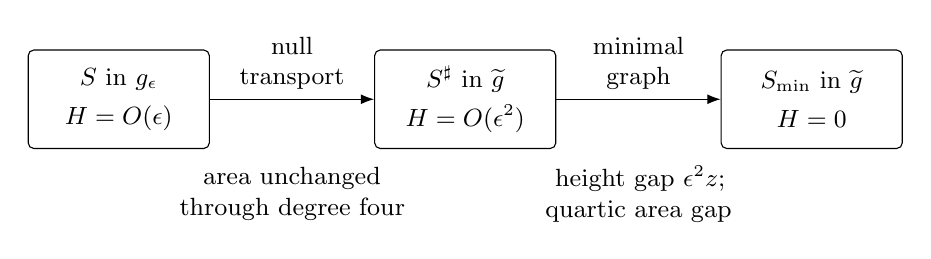
\begin{tikzpicture}[
  surface/.style={draw,rounded corners=2pt,align=center,
    minimum width=2.3cm,minimum height=1.25cm},
  >=Latex,font=\small]
 \node[surface] (original) at (0,0)
   {$S$ in $g_\eps$\\[3pt]$H=O(\eps)$};
 \node[surface] (cut) at (4.4,0)
   {$S^\sharp$ in $\widetilde g$\\[3pt]$H=O(\eps^2)$};
 \node[surface] (minimal) at (8.8,0)
   {$S_{\min}$ in $\widetilde g$\\[3pt]$H=0$};
 \draw[->] (original.east) -- (cut.west)
   node[midway,above,align=center]{null\\transport};
 \draw[->] (cut.east) -- (minimal.west)
   node[midway,above,align=center]{minimal\\graph};
 \node[align=center,text width=3.7cm] at (2.2,-1.2)
   {area unchanged\\through degree four};
 \node[align=center,text width=3.7cm] at (6.6,-1.2)
   {height gap $\eps^2z$;\\quartic area gap};
\end{tikzpicture}
\caption{The boundary comparisons in the changed slice.  The diagram
describes finite Taylor families, including the possibility of negative
leading displacements. The signed height gap is
$h^\sharp-h^{\min}=\eps^2z+O(\eps^3)$, and the corresponding area gap is
$|S^\sharp|_{\widetilde g}-|S_{\min}|_{\widetilde g}
=\frac12\eps^4\int_S zDz\,\dd A_{g_0}+O(\eps^5)$;
see \eqref{quart:area-hessian}. All displayed geometric statements are
understood through the required Taylor order.}
\label{fig:boundary-comparisons}
\end{figure}

Apply Proposition~\ref{prop:cmc-jets} to \(\widetilde g\) through
degree four.  Its hypotheses follow from
Lemma~\ref{lem:slice}, including the unchanged leading asymptotic
data.  Denote by \(f\) the lapse, by \(\bar f\) its area average on
each leaf, and set
\[
 \delta f=f-\bar f,\qquad
 U_j=[\II^{\tf}]_j,\qquad \mathcal F_j=[\delta f]_j.
\]
At degree two, the scalar contribution is zero by
\eqref{quart:scalar-four}.  Equations~\eqref{quart:null-area} and
\eqref{quart:area-hessian}, and the preserved mass, identify the
quadratic coefficient of mass minus \(b_*\) of the minimal-leaf area
with the original zero coefficient \(c_2[q]\).  The leading-energy
identity, Proposition~\ref{prop:leading-energy}, with its scalar
tensor equal to zero, gives
\[
 0=\frac1{16\pi}\int_M N
       \bigl(|U_1|^2+2\mathcal F_1J_s^0\mathcal F_1\bigr)\,\dd V_{g_0}.
\]
The lapse coefficient is mean free on each background sphere, and
\(J_s^0\) is strictly positive on that space.  Since \(N>0\) for
\(s>0\), sphere integration and smoothness imply
\begin{equation}
 U_1=0,\qquad \mathcal F_1=0.
 \label{quart:first-geometric-zero}
\end{equation}

We can now use Proposition~\ref{prop:leading-energy} at order four:
the scalar-curvature defect starts with
\(\eps^4|k|^2\), and both geometric square terms start in degree
four.  It follows first that mass minus \(b_*\) of the minimal-leaf
area has no coefficients below degree four.  The area correction
\eqref{quart:area-hessian} also starts in that degree.  Thus
\(c_3[q]=0\), as well as the previously known lower vanishings.

Let \(v_k\) be the decaying solution
\begin{equation}
 Lv_k=0,\qquad v_k|_S=z=D^{-1}(k_{ss}|_S).
 \label{quart:vk}
\end{equation}
It is supplied by Lemma~\ref{lem:inverse}.  The TT tensor \(k\) has
the decay and finite angular type required in
Lemma~\ref{lem:tt-square}.  Since
\(b_*'(4\pi a^2)=\kappa/(8\pi)\), subtracting the area correction
from the leading-energy identity and applying that lemma gives
\begin{equation}
 c_4[q]=\frac1{16\pi}\int_M N
   \left(
      |k-Q(v_k)|_{g_0}^2+|U_2|^2+2\mathcal F_2J_s^0\mathcal F_2
   \right)\,\dd V_{g_0}.
 \label{quart:square}
\end{equation}
Indeed the subtracted boundary term is exactly
\(\kappa(16\pi)^{-1}\int_S zDz\,\dd A_{g_0}\).
The integrals are understood with sphere integration first, as in
Proposition~\ref{prop:leading-energy}; no pointwise sign is asserted
for \(\mathcal F_2J_s^0\mathcal F_2\).  Its sphere integral is nonnegative.  This proves
\(c_4[q]\geq0\), and equality implies
\begin{equation}
 \delta f=O(\eps^3),\qquad
 \II^{\tf}=O(\eps^3)
 \label{quart:second-geometric-zero}
\end{equation}
on every leaf.  Boundary values follow by smoothness.  We show next
that \eqref{quart:second-geometric-zero} excludes a nonzero degree-one
part of \(v\).

\subsection{Round angular jets and conformal coordinates}
\label{quart:round-section}

We now assume equality in the quartic square. The vanishing in
\eqref{quart:second-geometric-zero} makes the changed metric a warped
product through degree two. The following lemma will round its angular
metric before we compare it with the conformal class of \(g_0\).

\Needspace{7\baselineskip}
\begin{lemma}[Rounding a two-jet on the sphere]
\label{lem:round-jet}
Let
\(\gamma_\eps=\sigma+\eps P_1+\eps^2P_2\) be a smooth metric
two-jet on \(S^2\) of finite angular type.  Suppose its scalar
curvature is angularly constant through degree two.  Then there are
a positive scalar two-jet \(a_\eps\), with \(a_0=1\), and a
diffeomorphism two-jet \(\Phi_\eps\), based at the identity, such that
\[
 \gamma_\eps=a_\eps\Phi_\eps^*\sigma+O(\eps^3).
\]
All coefficients can be chosen of finite angular type.
\end{lemma}

\begin{proof}
We first prove the infinitesimal decomposition used twice below.  For
a symmetric tensor \(P\) on the round sphere, there are a vector
field \(Y\) and a function \(h\) such that
\begin{equation}
 P=\mathcal L_Y\sigma+h\sigma.
 \label{quart:sphere-splitting}
\end{equation}
For finite-angular-type \(P\), the choices may retain that property.

Let \(P^{\tf}=P-\frac12(\tr_\sigma P)\sigma\), and identify vector
fields and one-forms using \(\sigma\).  Define
\[
 \mathcal C(Y)_{ij}
   =\nabla_iY_j+\nabla_jY_i-(\Div Y)\sigma_{ij}.
\]
On the curvature-one sphere, commuting covariant derivatives gives
\begin{equation}
 \Div\mathcal C(Y)=(\Delta_\sigma+1)Y,
 \qquad
 (\Delta_\sigma+1)\dd f=\dd(\Delta_\sigma+2)f.
 \label{quart:conformal-divergence}
\end{equation}
Here the Laplacian on one-forms is the rough Laplacian
\(\nabla^i\nabla_i\).
The second identity also holds after applying the parallel Hodge star
\(*\) to one-forms.

Put \(\alpha=\Div P^{\tf}\).  To decompose it, solve the scalar
equations
\[
 \Delta_\sigma\varphi=\Div\alpha,\qquad
 \Delta_\sigma\psi=-\Div(*\alpha)
\]
with zero means.  Both right sides have zero integral.  In finite
angular spaces these equations are solved by inversion on the
nonconstant spherical modes.  The residual
\(\omega=\alpha-\dd\varphi-*\dd\psi\) is closed and co-closed.
Commuting derivatives of a closed one-form of zero divergence gives
\(\nabla^i\nabla_i\omega=\omega\); integration against \(\omega\)
forces \(\omega=0\).  We have therefore obtained
\[
 \alpha=\dd\varphi+*\dd\psi.
\]

The one-forms \(\dd x_i\) and \(*\dd x_i\) correspond to conformal
Killing vector fields.  Integration by parts against the tracefree
tensor \(P^{\tf}\) consequently shows that \(\alpha\) is
orthogonal to all of them.  It follows that both \(\varphi\) and
\(\psi\) have zero degree-one components.  Thus we may solve
\[
 (\Delta_\sigma+2)A=\varphi,\qquad
 (\Delta_\sigma+2)C=\psi
\]
on their angular modes, and set \(Y^\flat=\dd A+*\dd C\).
Equation~\eqref{quart:conformal-divergence} gives
\(\Div\mathcal C(Y)=\Div P^{\tf}\).

The tracefree tensor \(P_*=P^{\tf}-\mathcal C(Y)\) is consequently
divergence free.  Such a tensor vanishes on the round sphere; here is
a direct verification.  In an orthonormal frame write its components
as
\(\left(\begin{smallmatrix}a&b\\b&-a\end{smallmatrix}\right)\).
Its two divergence equations are precisely the two independent
Codazzi equations
\(\nabla_i(P_*)_{jk}=\nabla_j(P_*)_{ik}\).
Contracting and commuting these equations on the curvature-one sphere
gives
\[
 \nabla^i\nabla_i(P_*)_{jk}
      =2(P_*)_{jk}-\sigma_{jk}\tr_\sigma P_*
      =2(P_*)_{jk}.
\]
Integration yields
\(-\int|\nabla P_*|^2=2\int|P_*|^2\), hence \(P_*=0\).
Taking
\(h=\frac12\tr_\sigma P-\Div Y\) proves
\eqref{quart:sphere-splitting}.  Every operation used above commutes
with rotations or inverts a scalar operator within finitely many
spherical eigenspaces, so it preserves finite angular type.

The scalar-curvature derivative in the direction \(h\sigma\) is
\[
 (D\scal)_\sigma(h\sigma)=-\Delta_\sigma h-2h.
\]
The derivative in a Lie direction is zero because the background
scalar curvature is constant.  If the scalar-curvature variation of
\(P\) is constant, \eqref{quart:sphere-splitting} therefore implies
that \(h\) consists only of a constant and degree-one modes.  A
degree-one function \(h_1\) satisfies
\(\Hess_\sigma h_1=-h_1\sigma\), so
\[
 h_1\sigma
   =\mathcal L_{-\frac12\grad_\sigma h_1}\sigma.
\]
Thus \(P\) is a Lie derivative plus a constant multiple of \(\sigma\).

Apply this conclusion to \(P_1\).  A formal inverse flow and a scalar
scaling remove its first coefficient.  Both operations preserve
the property that curvature is angularly constant.  The resulting
metric two-jet has the form \(\sigma+\eps^2\widehat P_2\), so its
degree-two curvature equation is the same linearized equation, with
no quadratic contribution from a first coefficient.  The argument
just given removes \(\widehat P_2\) by a degree-two flow and scaling.
Undoing the two operations proves the stated rounding.  This proves
only an identity of two-jets, which is exactly what is required.
\end{proof}

\paragraph{Local conformal tangency forced by equality.}
Suppose now that \(c_4[q]=0\). Fix a compact interval
\(I\Subset(0,\infty)\).  In coordinates of the CMC sphere jets we can
remove tangential shift through degree two by integrating its
tangential reparametrization equation on \(I\).  Its background
value is zero, so the coordinate change is based at the identity.
In these coordinates \eqref{quart:second-geometric-zero} says that the
lapse is a function of the leaf parameter only and that
\(\II=(H/2)g_{\rm leaf}\) through degree two.  Since \(H\) is
constant on each leaf, the normal metric variation is
\[
 \partial_s g_{\rm leaf}=2f\II=fH g_{\rm leaf}.
\]
Consequently on \(I\times S^2\) the metric has the form
\begin{equation}
 f_*(s)^2\dd s^2+b(s)^2\gamma_\eps(x)+O(\eps^3),
 \label{quart:warped-two}
\end{equation}
where all quantities are two-jets, with backgrounds \(f_*=1\),
\(b=r\), and \(\gamma_0=\sigma\).  Angular finiteness is preserved
by these Taylor coordinate changes and integrations.

For this warped metric the scalar curvature through degree two is
\begin{equation}
 b^{-2}\scal_{\gamma_\eps}
   -\frac4{f_*b}\frac{\dd}{\dd s}
                      \left(\frac{b'}{f_*}\right)
   -2\left(\frac{b'}{f_*b}\right)^2.
 \label{quart:warped-scalar}
\end{equation}
Equation~\eqref{quart:scalar-four} makes it the constant \(-6\)
through degree two.  The last two terms in
\eqref{quart:warped-scalar} are radial, so
\(\scal_{\gamma_\eps}\) is angularly constant to that order.
Lemma~\ref{lem:round-jet} makes \(\gamma_\eps\) round up to
diffeomorphism and scaling.  Absorbing the scaling into \(b\), we
obtain \(f_*^2\dd s^2+b^2\sigma\).

This last two-jet is locally conformal to a pullback of \(g_0\).
Indeed solve, coefficientwise on \(I\),
\begin{equation}
 \frac{y'}{r(y)}=\frac{f_*}{b},
 \label{quart:radial-coordinate}
\end{equation}
with background \(y=s\) and a fixed identity background initial value
at an interior point of \(I\).  This is a nonsingular scalar ODE,
and it gives
\[
 f_*^2\dd s^2+b^2\sigma
   =\frac{b^2}{r(y)^2}
       \bigl(\dd y^2+r(y)^2\sigma\bigr)
       \quad\bmod\eps^3.
\]
Composing the coordinate changes already made shows, in the original
coordinates on the interval, that
\begin{equation}
 \widetilde g=\omega_\eps\Psi_\eps^*g_0+O(\eps^3),
 \qquad \omega_0=1,\quad\Psi_0=\mathrm{id}.
 \label{quart:conformal-pullback}
\end{equation}
Only this local statement is used.

There is a useful consequence of the known first coefficient in
\eqref{quart:conformal-pullback}.  Write
\(\omega_\eps=1+\eps a_1+\eps^2a_2\) and express the
diffeomorphism two-jet as
\[
 \Psi_\eps^*g_0
  =g_0+\eps\mathcal L_Xg_0
      +\eps^2\bigl(\mathcal L_Zg_0
                      +\tfrac12\mathcal L_X^2g_0\bigr).
\]
The graph calculation shows that \(\widetilde g-g_\eps\) starts
in degree two, so \([\widetilde g]_1=4ug_0\).  Hence
\(\mathcal L_Xg_0=\lambda g_0\) for some function \(\lambda\).
It follows that
\[
 \mathcal L_X^2g_0=(X\lambda+\lambda^2)g_0,
\]
and the mixed scalar term \(a_1\mathcal L_Xg_0\) is pure trace as
well.  Therefore
\begin{equation}
 [\widetilde g]_2=\mathcal L_Zg_0+c g_0
 \label{quart:second-tangent}
\end{equation}
for a function \(c\) on \(I\times S^2\).  The original metric
coefficient \([g_\eps]_2\) is itself pure trace.  Thus the same
Lie-derivative-plus-trace conclusion holds for their difference.
Since \(\Hess(v^2)=\frac12\mathcal L_{\grad(v^2)}g_0\),
\eqref{quart:metric-two} gives the necessary condition
\begin{equation}
 \dd v\otimes\dd v+Bv^2=\mathcal L_Yg_0+c g_0
 \quad\hbox{on }I\times S^2
 \label{quart:necessary-tangent}
\end{equation}
for some local \(Y,c\).  Their choices may depend on \(I\).

\subsection{The degree-one obstruction}\label{quart:obstruction-section}

\begin{lemma}[A nonzero degree-one mode is obstructed]
\label{lem:dipole-obstruction}
Let \(v=v_0(s)+V(s)x\) solve \(Lv=0\), where \(x\) is one fixed
unit-axis linear coordinate on \(S^2\) and \(V=O(r^{-3})\).
If \eqref{quart:necessary-tangent} holds on every compact radial
interval in the interior, with possibly different local vector fields
and functions, then \(V\equiv0\).
\end{lemma}

\begin{proof}
Set \(Y_2=x^2-1/3\), a degree-two spherical eigenfunction.  Project
\eqref{quart:necessary-tangent} onto its scalar, gradient, and
tangential Hessian modes.  Write the contributing radial vector-field
coefficient as \(p(s)Y_2\partial_s\), its tangential coefficient as
\(d(s)\grad_\sigma Y_2\), and the scalar-multiple coefficient as
\(c(s)Y_2\).  These are the only generator components contributing to
the tested modes.  This follows either from the one-form decomposition
in Lemma~\ref{lem:round-jet} or by integration by parts, using
\(\Delta_\sigma Y_2=-6Y_2\).  In particular, the coexact component
is orthogonal to both the gradient test and the electric Hessian
test, and the other spherical eigenspaces are orthogonal as well.

For clarity, the angular identity
\[
 \dd x\otimes\dd x
       =\tfrac12\Hess_\sigma Y_2+x^2\sigma
\]
shows all terms of the left side in these modes.  With
\(B=B_s\dd s^2+B_t r^2\sigma\), equality of the radial, mixed,
Hessian, and tangential scalar coefficients respectively gives
\begin{align}
 V'^2+B_sV^2&=2p'+c,
 &\frac{VV'}2&=p+r^2d',\nonumber\\
 \frac{V^2}2&=2r^2d,
 &V^2+r^2B_tV^2&=2rNp+r^2c.
 \label{quart:projection-system}
\end{align}
Terms involving \(v_0\) have only degrees zero or one and do not
enter these equations.  Solving the last three equations yields
\[
 d=\frac{V^2}{4r^2},\qquad
 p=\frac{NV^2}{2r},\qquad
 c=\frac{3m_0V^2}{r^3}.
\]
Substitute these expressions in the first equation and use
\[
 B_s=1-\frac{2m_0}{r^3},\qquad
 B_t=1+\frac{m_0}{r^3},\qquad
 N'=r+\frac{m_0}{r^2},\qquad
 N^2=1+r^2-\frac{2m_0}{r}.
\]
After cancellation one obtains
\begin{equation}
 \left(V'-\frac NrV\right)^2
       =\frac{6m_0}{r^3}V^2.
 \label{quart:dipole-identity}
\end{equation}
The local generators have disappeared from this relation.  Because
the radial interval was arbitrary, it holds throughout the end even
though their choices need not agree on overlapping intervals.

For \(z=V/r\), \eqref{quart:dipole-identity} reads
\[
 |z'|=\sqrt{6m_0}\,r^{-3/2}|z|.
\]
The coefficient on the right is integrable toward infinity, and
\(z\to0\).  The integral differential inequality, applied backwards
between \(s\) and \(S>s\), gives
\[
 |z(s)|\leq |z(S)|
       \exp\left(\int_s^S\sqrt{6m_0}\,r(t)^{-3/2}\,\dd t\right).
\]
Letting \(S\to\infty\) proves \(z=0\) on the end.  The homogeneous
degree-one ODE obtained from \(Lv=0\) then gives \(V\equiv0\) by
uniqueness.
\end{proof}

\begin{proof}[Completion of the proof of Proposition~\ref{prop:quartic}]
The coefficient vanishings and nonnegativity were proved in
\eqref{quart:first-geometric-zero}--\eqref{quart:square}.  Suppose
that the degree-one part of \(v\) is nonzero and that \(c_4[q]=0\).
All three degree-one radial coefficients solve the same decaying
homogeneous ODE.  Decaying uniqueness makes them proportional, so
after a fixed rotation their sum is \(V(s)x\) for one axis and a
nonzero radial function \(V\).  The vanishing consequences of
\eqref{quart:square} give \eqref{quart:necessary-tangent} on each
interior radial interval.  Lemma~\ref{lem:dipole-obstruction} forces
\(V=0\), a contradiction.  Thus \(c_4[q]>0\).

Finally this is a statement about the actual deficit, not only a
formal inequality.  The kernel representation gives precisely the
finite angular type and differentiated decay needed for the
fourth-order expansion in Proposition~\ref{prop:expansions}.
Lemma~\ref{lem:green} converts the weighted function and equation
remainders to the mass remainder.  Consequently
\[
 \mathfrak D_q(\eps)=c_4[q]\eps^4+O(\eps^5)
\]
in the case under consideration.  Its positive coefficient gives
strict positivity for all sufficiently small positive \(\eps\),
with the interval allowed to depend on the fixed data.  The radial
kernel, including the zero seed, is handled by the exact argument in
the next section.
\end{proof}

\section{Radial equality and the nonlinear conclusion}
\label{sec:conclusion}

\begin{proposition}[Exact radial equality]
\label{prop:radial}
Suppose the fixed TT seed $q$ is invariant under rotations of $S^2$.
Every branch in Theorem~\ref{thm:main} is radial for all sufficiently
small $\eps$, and on that parameter interval
\[
 m_{\AH}(\eps)=b_*(A_\eps).
\]
This includes the zero seed, and requires no sign for $q_{ss}|_S$.
\end{proposition}

\begin{proof}
We first prove radiality of the actual solution, rather than merely
of its Taylor coefficients.  Fix a rotation $\mathcal R$, and set
$\widehat\phi=\phi_\eps\circ\mathcal R$ and
$w=\widehat\phi-\phi_\eps$.
Because $q$ is radial, $\widehat\phi$ satisfies the same equation and
boundary condition as $\phi_\eps$.  Their difference satisfies
\begin{equation}
 (\Delta_{g_0}-c_\eps)w=0,
 \qquad w_s|_S=c_\eps^*w|_S,
 \label{eq:radial-uniqueness-equation}
\end{equation}
where divided differences of the nonlinearities give, uniformly on
$M$ and uniformly in $\mathcal R$,
\[
 c_\eps=3+o(1),\qquad c_\eps^*=O(\eps).
\]
Indeed, the derivatives of the interior and boundary nonlinearities
with respect to their positive scalar argument $z$ are respectively
\[
 \frac34(5z^4-1)+\frac{7\eps^2}{8}|q|^2z^{-8},
 \qquad -\frac{3\eps}{4}q_{ss}z^{-4}.
\]
The asserted bounds follow from boundedness of $q$ and the given
uniform convergence $\phi_\eps\to1$.

Choose $3/2<\beta<\min(\tau,\sqrt3)$. Then
$w=o(e^{-\beta s})$, and \eqref{eq:radial-uniqueness-equation} has the
form of Lemma~\ref{lem:inverse} with $V=c_\eps-3$, Robin coefficient
$a_*=c_\eps^*$, and zero interior and boundary data. For sufficiently
small $\eps$, uniformly in the rotation, $\|V\|_\infty\leq c_\beta$
and $\|a_*\|_\infty\leq\beta/2$. The comparison estimate gives $w=0$,
so the actual $\phi_\eps$ is radial.

Write the invariant seed as
$q=A_q(s)\,\dd s^2+B_q(s)r^2\sigma$.
Its trace and divergence equations give
\[
 B_q=-A_q/2,
 \qquad A_q'+3(N/r)A_q=0.
\]
Consequently, for a constant $C_q\in\mathbb R$,
\begin{equation}
 q=C_qr^{-3}\left(\dd s^2-\frac12r^2\sigma\right).
 \label{eq:radial-tt-tensor}
\end{equation}
Fix a sufficiently small parameter.  Define proper radial distance
$\ell$ and the actual area radius $R$ by
\[
 \dd\ell=\phi_\eps^2\,\dd s,
 \qquad R=r\phi_\eps^2.
\]
Then the actual metric and second-form data are
\[
 g_\eps=\dd\ell^2+R^2\sigma,
 \qquad K_\eps=-2k\,\dd\ell^2+kR^2\sigma,
 \qquad k=-\frac{\eps C_q}{2R^3}.
\]
A dot denotes an $\ell$-derivative.  The momentum and scalar constraints
are therefore
\begin{equation}
 \dot k=-3\frac{\dot R}{R}k,
 \qquad
 -\frac{4\ddot R}{R}
 +\frac{2(1-\dot R^2)}{R^2}+6=6k^2.
 \label{eq:radial-constraints}
\end{equation}
The scalar-curvature formula here follows from the sectional curvatures
$-\ddot R/R$ and $(1-\dot R^2)/R^2$ of this warped product.

Define
\begin{equation}
 \mathcal M
 =\frac R2\left(1+R^2-\dot R^2+R^2k^2\right).
 \label{eq:radial-conserved-mass}
\end{equation}
Direct differentiation, using the momentum equation, gives
\[
 \dot{\mathcal M}
 =\frac{\dot R}{2}
 \left(1+3R^2-\dot R^2-2R\ddot R-3R^2k^2\right)=0
\]
by the scalar equation in \eqref{eq:radial-constraints}.
No division by $\dot R$ has been used, so conservation is valid at
turning points of $R$ as well.
At the boundary the MOTS equation reads
\[
 \frac{2\dot R}{R}+2k=0.
\]
Substitution in \eqref{eq:radial-conserved-mass} yields
\begin{equation}
 \mathcal M|_S
 =\frac{R|_S}{2}\bigl(1+(R|_S)^2\bigr)
 =b_*\bigl(4\pi(R|_S)^2\bigr)=b_*(A_\eps).
 \label{eq:radial-mass-at-boundary}
\end{equation}

We identify the same constant with the specified mass flux at infinity.
Put $\psi=\phi_\eps-1$.  Its actual radial equation gives
\[
 \psi''+2\frac Nr\psi'-3\psi
 =O(\psi^2)+O(r^{-6}),
\]
where \eqref{eq:radial-tt-tensor} was used in the source estimate.
The assumed weighted decay gives
$\psi,\psi'=O(e^{-\tau s})$, and $N/r=1+O(e^{-2s})$.
It follows that
\[
 \psi''+2\psi'-3\psi=O(e^{-\gamma s}),
 \qquad \gamma=\min(2\tau,\tau+2,6)>3.
\]
Variation of constants for the roots $1,-3$ excludes the growing
solution by the prescribed decay and yields, as in
Lemma~\ref{lem:inverse}, a constant $c=c(\eps)$ with
\begin{equation}
 \phi_\eps=1+cr^{-3}+o(r^{-3}),
 \qquad
 \partial_s\phi_\eps=-3cNr^{-4}+o(r^{-3}).
 \label{eq:radial-actual-asymptotic}
\end{equation}
In particular,
\[
 R=r+2cr^{-2}+o(r^{-2}),\qquad
 \dot R=N+2r\frac{\partial_s\phi_\eps}{\phi_\eps}
 =N-6cNr^{-3}+o(r^{-2}).
\]
Using $N^2=1+r^2-2m_0/r$, we obtain
\[
 1+R^2-\dot R^2
 =\frac{2m_0+16c}{r}+o(r^{-1}).
\]
Also $R^3k^2=O(R^{-3})$, so
\begin{equation}
 \lim_{\ell\to\infty}\mathcal M=m_0+8c.
 \label{eq:radial-mass-at-infinity}
\end{equation}

For a direct flux normalization check, rotational invariance implies
$p_i=0$ for $i=1,2,3$.
Equation~\eqref{eq:radial-actual-asymptotic} implies
\[
 g_\eps-g_0=4cr^{-3}b+o(r^{-3})
\]
in scaled components, with its first differentiated asymptotic.
For a perturbation $fb$ in dimension three, the mass-flux covector
integrand with test function $V$ simplifies to
$2(f\,\dd V-V\,\dd f)$.
With $f=4cr^{-3}$, $V=V_0=\sqrt{1+r^2}$, and
$\nu_b=\sqrt{1+r^2}\,\partial_r$, its normal component is
\[
 2\bigl(f\partial_{\nu_b}V_0
       -V_0\partial_{\nu_b}f\bigr)
 =32cr^{-2}+24cr^{-4}.
\]
The error terms give zero limiting flux.  Integrating over a coordinate
sphere of area $4\pi r^2$ and dividing by $16\pi$ gives
$p_0-m_0=8c$.
Since $p_0\to m_0>0$ as $\eps\to0$,
\[
 m_{\AH}=p_0=m_0+8c=\mathcal M=b_*(A_\eps)
\]
for sufficiently small $\eps$, by
\eqref{eq:radial-mass-at-boundary}--\eqref{eq:radial-mass-at-infinity}.
This argument includes $C_q=0$.  In that case one can also apply the
comparison estimate of Lemma~\ref{lem:inverse} to $\phi_\eps-1$
and conclude $\phi_\eps\equiv1$ directly.
\end{proof}

\begin{proof}[Completion of the proof of Theorem~\ref{thm:main}]
Fix the seed and the given solution branch.  If $q$ is radial,
Proposition~\ref{prop:radial} gives exact equality on a sufficiently
small parameter interval.
Suppose henceforth that $q$ is not radial.
Proposition~\ref{prop:quadratic} gives the actual expansion
\[
 \mathfrak D_q(\eps)=c_2[q]\eps^2+o(\eps^2),
 \qquad c_2[q]\geq0.
\]
If $c_2[q]>0$, this proves strict positivity of the deficit for every
sufficiently small positive $\eps$.

If $c_2[q]=0$, Corollary~\ref{cor:kernel} gives
$q=Q(v)$ with $Lv=0$ and with only constant and linear angular modes.
Its linear part is nonzero, for otherwise $q$ would be radial.
These homogeneous modes have the stronger differentiated decay needed
for the actual fourth-order expansion in
Proposition~\ref{prop:expansions}.
Proposition~\ref{prop:quartic} then gives
\[
 \mathfrak D_q(\eps)=c_4[q]\eps^4+o(\eps^4),
 \qquad c_4[q]>0,
\]
with all coefficients below order four equal to zero.
Again the actual deficit is strictly positive for every sufficiently
small positive $\eps$.

At $\eps=0$ the background identity
$m_0=b_*(4\pi a^2)$ gives equality.
The preceding alternatives exhaust all fixed seeds.  Choose
$\eps_0>0$ small enough for the applicable alternative and the given
branch, with $\eps_0\leq\eps_*$.
This proves the exact inequality on $0\leq\eps<\eps_0$, equality for
radial seeds, and strict inequality for nonradial seeds at positive
parameters in that interval.
The size of the interval is allowed to depend on the fixed seed and
branch; no uniform positive lower bound for $c_2$ or $c_4$ is asserted
or required.
\end{proof}

\clearpage
\bibliographystyle{support/alpha-linked}
\bibliography{refs}
\end{document}
